\part{杂项与工具}

\chapter{其他算法}

\section{莫队}
\entrymeta{$O((n+m)\sqrt n)$}
\subsection{P1494 {[}国家集训队{]} 小 Z 的袜子}\label{p1494-ux56fdux5bb6ux96c6ux8badux961f-ux5c0f-z-ux7684ux889cux5b50}


\begin{codeline}
const int N = 50005;
int S = 250;

long long gcd(long long A, long long B) {
    return B == 0 ? A : gcd(B, A % B);
}

class Query {
public:
    int l, r;
    long long ans;
    bool operator<(const Query& o) const {
        if(l / S != o.l / S) {
            return l / S < o.l / S;
        } else {
            return (l / S) & 1 ? r < o.r : r > o.r;
            ;
        }
    }
};

Query q[N];
int ptr[N];

bool cmp(const int A, const int B) {
    return q[A] < q[B];
}

int a[N];
int cnt[N];

int main() {
    ios::sync_with_stdio(false);
    cin.tie(nullptr);
    int n, m;
    cin >> n;
    cin >> m;
    S = max(1, int(n / sqrt(max(1, m))));
    for(int i = 1; i <= n; i++) {
        cin >> a[i];
    }
    for(int i = 1; i <= m; i++) {
        cin >> q[i].l;
        cin >> q[i].r;
        ptr[i] = i;
    }
\end{codeline}
\vspace{-0.9\baselineskip}
\begin{codeline}[firstnumber=47]
    sort(ptr + 1, ptr + 1 + m, cmp);

    int l = 1, r = 1;
    long long ans = 0;
    cnt[a[1]]++;
    for(int i = 1; i <= m; i++) {
        Query& query = q[ptr[i]];
        while(l > query.l) {
            ans += cnt[a[--l]]++;
        }
        while(r < query.r) {
            ans += cnt[a[++r]]++;
        }
        while(l < query.l) {
            ans -= --cnt[a[l++]];
        }
        while(r > query.r) {
            ans -= --cnt[a[r--]];
        }
        query.ans = ans;
    }

    for(int i = 1; i <= m; i++) {
        if(q[i].ans == 0) {
            cout << "0/1\n";
        } else {
            long long tot = (q[i].r - q[i].l + 1ll) * (q[i].r - q[i].l) / 2;
            long long g = gcd(q[i].ans, tot);
            cout << (q[i].ans / g) << "/" << (tot / g) << '\n';
        }
    }
}
\end{codeline}


\subsection{P1903 {[}国家集训队{]} 数颜色 / 维护队列 /【模板】带修莫队}\label{p1903-ux56fdux5bb6ux96c6ux8badux961f-ux6570ux989cux8272-ux7ef4ux62a4ux961fux5217-ux6a21ux677fux5e26ux4feeux83abux961f}


\begin{codeline}
const int N = 140005;
const int C = 1000005;
int S = 400;

class Query {
public:
    int l, r, t;
    long long ans;
    bool operator<(const Query& o) const {
        if(l / S != o.l / S) {
            return l / S < o.l / S;
        } else if(r / S != o.r / S) {
            return r / S < o.r / S;
        } else {
            return (r / S) & 1 ? t < o.t : t > o.t;
            ;
        }
    }
};

Query q[N];
int qcnt;
int ptr[N];
int mod[N][3];

bool cmp(const int A, const int B) {
    return q[A] < q[B];
}

int a[N];
int cnt[C];

int main() {
    int n, m;
    cin >> n >> m;
    S = pow(n, 0.66);
    for(int i = 1; i <= n; i++) {
        cin >> a[i];
    }
    int t = 0;
    int l = 1, r = 1;
    long long ans = 0;
    char op;
    for(int i = 1; i <= m; i++) {
        cin >> op >> l >> r;
        if(op == 'Q') {
\end{codeline}
\vspace{-0.9\baselineskip}
\begin{codeline}[firstnumber=47]
            q[++qcnt] = {l, r, t};
            ptr[qcnt] = qcnt;
        } else {
            mod[t][0] = l;
            mod[t][1] = a[l];
            mod[t][2] = r;
            a[l] = r;
            ++t;
        }
    }
    sort(ptr + 1, ptr + 1 + qcnt, cmp);

    l = r = 1;
    cnt[a[1]]++;
    ans = 1;

    for(int i = 1; i <= qcnt; i++) {
        Query& query = q[ptr[i]];
        while(l > query.l) {
            --l;
            if(cnt[a[l]] == 0) {
                ans++;
            }
            cnt[a[l]]++;
        }
        while(r < query.r) {
            ++r;
            if(cnt[a[r]] == 0) {
                ans++;
            }
            cnt[a[r]]++;
        }
        while(l < query.l) {
            cnt[a[l]]--;
            if(cnt[a[l]] == 0) {
                ans--;
            }
            l++;
        }
        while(r > query.r) {
            cnt[a[r]]--;
            if(cnt[a[r]] == 0) {
                ans--;
            }
            r--;
        }
\end{codeline}
\vspace{-0.9\baselineskip}
\begin{codeline}[firstnumber=93]
        while(t < query.t) {
            if(mod[t][0] >= l && mod[t][0] <= r) {
                cnt[mod[t][1]]--;
                if(cnt[mod[t][1]] == 0) {
                    ans--;
                }
                if(cnt[mod[t][2]] == 0) {
                    ans++;
                }
                cnt[mod[t][2]]++;
            }
            a[mod[t][0]] = mod[t][2];
            ++t;
        }
        while(t > query.t) {
            --t;
            if(mod[t][0] >= l && mod[t][0] <= r) {
                cnt[mod[t][2]]--;
                if(cnt[mod[t][2]] == 0) {
                    ans--;
                }
                if(cnt[mod[t][1]] == 0) {
                    ans++;
                }
                cnt[mod[t][1]]++;
            }
            a[mod[t][0]] = mod[t][1];
        }
        query.ans = ans;
    }

    for(int i = 1; i <= qcnt; i++) {
        cout << (q[i].ans) << '\n';
    }
}
\end{codeline}
\begin{warnbox}
块长取 \texttt{max(1, n / sqrt(m))}，防止 m 很大时除零；\texttt{ptr} 要初始化到 m。
\end{warnbox}

\section{环计数}
\entrymeta{$O(m\sqrt m)$}
\subsection{P1989 无向图三元环计数}\label{p1989-ux65e0ux5411ux56feux4e09ux5143ux73afux8ba1ux6570}










\begin{codeline}
const int N = 100005;

class Node {
public:
    vector<int> oe;
    int degree;
    bool visited;
};

Node node[N];

int n, m;

int main() {
    ios::sync_with_stdio(false);
    cin.tie(nullptr);
    cin >> n >> m;
    set<int> nidx;
    vector<pair<int, int>> edge;
    for(int i = 0; i < m; i++) {
        int u, v;
        cin >> u >> v;
        edge.push_back({u, v});
        node[u].degree++;
        node[v].degree++;
        nidx.insert(u);
        nidx.insert(v);
    }

    for(pair<int, int> e : edge) {
        if(node[e.first].degree > node[e.second].degree || (node[e.first].degree == node[e.second].degree && e.first > e.second)) {
            node[e.first].oe.push_back(e.second);
        } else {
            node[e.second].oe.push_back(e.first);
        }
    }

    int ans = 0;

    for(int u : nidx) {
        for(int v : node[u].oe) {
            node[v].visited = true;
        }
        for(int v : node[u].oe) {
            for(int w : node[v].oe) {
                if(node[w].visited) {
\end{codeline}
\vspace{-0.9\baselineskip}
\begin{codeline}[firstnumber=47]
                    ans++;
                }
            }
        }
        for(int v : node[u].oe) {
            node[v].visited = false;
        }
    }

    cout << (ans) << '\n';
}
\end{codeline}


\subsection{题意精炼}\label{ux9898ux610fux7cbeux70bc}

给定一个无向图，有 \(n\) 个节点（城镇）和 \(m\) 条边（铁路连接）。每条边的权重为 \(a\)。此外，对于图中任意两个节点 \(u\) 和 \(v\)，如果它们没有直接边相连，但存在一个公共邻居 \(w\)（即存在边 \((u,w)\) 和 \((w,v)\)），则添加一条边 \((u,v)\)，权重为 \(b\)。

现在，给定源节点 \(k\)，要求计算从 \(k\) 到每个节点的最短路径成本。注意，从 \(k\) 到自身的成本为 \(0\)。


\begin{codeline}
const int N = 100005;

int n, m, k, a, b;

class Node {
public:
    vector<int> sub;
    vector<int> leap;
    int dis;
    int even_dis;
    bool visited;
    bool flag;
};

Node node[N];

int main() {
    ios::sync_with_stdio(false);
    cin.tie(nullptr);
    cin >> n >> m >> k >> a >> b;
    for(int i = 0; i < m; i++) {
        int u, v;
        cin >> u >> v;
        node[u].sub.push_back(v);
        node[v].sub.push_back(u);
    }

    for(int i = 0; i <= n; i++) {
        node[i].leap = vector<int>(node[i].sub);
        node[i].dis = 0x3f3f3f3f;
        node[i].even_dis = 0x3f3f3f3f;
    }

    node[k].dis = 0;
    node[k].visited = true;
    queue<int> q;
    q.push(k);
    int u;
    while(!q.empty()) {
        u = q.front();
        q.pop();

        for(int v : node[u].sub) {
            if(!node[v].visited) {
                node[v].dis = node[u].dis + 1;
                node[v].visited = true;
\end{codeline}
\vspace{-0.9\baselineskip}
\begin{codeline}[firstnumber=47]
                q.push(v);
            }
        }
    }

    if(b < 2 * a) {
        node[k].even_dis = 0;
        q.push(k);
        node[k].visited = false;
        while(!q.empty()) {
            u = q.front();
            q.pop();
            for(int v : node[u].leap) {
                node[v].flag = true;
            }
            for(int v : node[u].sub) {
                vector<int> remained;
                remained.reserve(node[v].leap.size());

                for(int w : node[v].leap) {
                    if(node[w].visited && !node[w].flag) {
                        node[w].even_dis = node[u].even_dis + 2;
                        node[w].visited = false;
                        q.push(w);
                    } else {
                        remained.push_back(w);
                    }
                }
                node[v].leap = remained;
            }
            for(int v : node[u].leap) {
                node[v].flag = false;
            }
        }

        for(int i = 1; i <= n; i++) {
            cout << (min((node[i].dis % 2) * a + node[i].dis / 2 * b, node[i].even_dis != 0x3f3f3f3f ? node[i].even_dis / 2 * b : 0x3f3f3f3f)) << '\n';
        }
    } else {
        for(int i = 1; i <= n; i++) {
            cout << (node[i].dis * a) << '\n';
        }
    }
}
\end{codeline}
\begin{warnbox}
按度数定向；不可达判 \texttt{!= INF}，不要用 \texttt{\textless{}= n}。
\end{warnbox}

\section{分数规划}
\entrymeta{$O(n\log n)$ 每次判定}
分数规划用来求一个分式的极值。

形象一点就是，给出 \(a_i\) 和 \(b_i\)，求一组 \(w_i\in\{0,1\}\)，最小化或最大化

\[
\displaystyle\frac{\sum\limits_{i=1}^na_i\times w_i}{\sum\limits_{i=1}^nb_i\times w_i}
\]

另外一种描述：每种物品有两个权值 \(a\) 和 \(b\)，选出若干个物品使得 \(\displaystyle\frac{\sum a}{\sum b}\) 最小/最大。

一般分数规划问题还会有一些奇怪的限制，比如『分母至少为 \(W\)』。

\subsection{求解}\label{ux6c42ux89e3}

\subsubsection{二分法}\label{ux4e8cux5206ux6cd5}

分数规划问题的通用方法是二分。

假设我们要求最大值。二分一个答案 \(mid\)，然后推式子（为了方便少写了上下界）：

\[
\displaystyle
\begin{aligned}
&\frac{\sum a_i\times w_i}{\sum b_i\times w_i}>mid\\
\Longrightarrow&\sum a_i\times w_i-mid\times \sum b_i\cdot w_i>0\\
\Longrightarrow&\sum w_i\times(a_i-mid\times b_i)>0
\end{aligned}
\]

那么只要求出不等号左边的式子的最大值就行了。如果最大值比 \(0\) 要大，说明 \(mid\) 是可行的，否则不可行。

\subsection{P4377 {[}USACO18OPEN{]} Talent Show G}\label{p4377-usaco18open-talent-show-g}






\begin{codeline}
const double eta = 1e-8;
int n, W;
double p[256];
int w[256];
double dp[1024];
int main() {
    ios::sync_with_stdio(false);
    cin.tie(nullptr);
    cin >> n >> W;
    for(int i = 1; i <= n; i++) {
        cin >> w[i] >> p[i];
    }

    double l = 0, r = 1e7, mid = 0.0, sum_w, ans = 0.0;
    while(r - l > eta) {
        mid = (l + r) / 2;
        for(int k = 0; k <= W; k++) {
            dp[k] = -1e32;
        }
        dp[0] = 0;

        bool flag = false;

        for(int i = 1; i <= n; i++) {
            for(int j = W + w[i]; j >= w[i]; j--) {
                int k = min(j, W);
                dp[k] = max(dp[k], dp[j - w[i]] + p[i] - mid * w[i]);
                if(dp[W] > eta) {
                    flag = true;
                    break;
                }
            }
            if(flag) {
                break;
            }
        }
        if(flag) {
            ans = mid;
            l = mid;
        } else {
            r = mid;
        }
    }

    cout << (int((ans + eta * 10) * 1000));
}
\end{codeline}
\begin{warnbox}
二分答案后转成判定性问题。
\end{warnbox}

\section{梯度下降}
\entrymeta{迭代次数 × $O(n)$}
\subsection{P1337 {[}JSOI2004{]} 平衡点 / 吊打XXX}\label{p1337-jsoi2004-ux5e73ux8861ux70b9-ux540aux6253xxx}






\begin{codeline}
const double ETA = 1e-4;
const int N = 1024;
double lr = 1e-3;
const double alpha = 0.9;
class Vec {
public:
    double x, y;
    Vec operator+(const Vec& o) const {
        return {x + o.x, y + o.y};
    }

    Vec operator*(double a) const {
        return {x * a, y * a};
    }

    double len() const {
        return sqrt(x * x + y * y);
    }
};

int n;
int X[N], Y[N], W[N];

Vec getForce(double x, double y, int b) {
    double dx = X[b] - x;
    double dy = Y[b] - y;
    double l = sqrt(dx * dx + dy * dy);
    if(l > ETA) {
        return {W[b] * dx / l, W[b] * dy / l};
    } else {
        return {0, 0};
    }
}

Vec totForce(const Vec& p) {
    Vec f = {0, 0};
    for(int i = 1; i <= n; i++) {
        f = f + getForce(p.x, p.y, i);
    }
    return f;
}

int main() {
    ios::sync_with_stdio(false);
    cin.tie(nullptr);
    cin >> n;
\end{codeline}
\vspace{-0.9\baselineskip}
\begin{codeline}[firstnumber=47]
    double sum = 0, sx = 0, sy = 0;
    for(int i = 1; i <= n; i++) {
        cin >> X[i] >> Y[i] >> W[i];
        sum += W[i];
        sx += X[i] * W[i];
        sy += Y[i] * W[i];
    }

    int cnt = 0;
    Vec p = {sx / sum, sy / sum};
    Vec f = {0, 0};
    while(++cnt) {
        f = f * alpha + totForce(p) * (1 - alpha); //动量梯度下降
        if(f.len() < ETA) {
            break;
        } else {
            p = p + f * lr;
        }
    }

    cout << fixed << setprecision(3) << (p.x) << ' ' << fixed << setprecision(3) << (p.y) << '\n';
}
\end{codeline}
\begin{warnbox}
步长与迭代上限要写死，否则可能在合法数据上不收敛。
\end{warnbox}

\section{高精度}
\entrymeta{$O(n^2)$}
\begin{codeline}
struct BigInt {
    int sign;
    vector<int> v;

    BigInt() : sign(1) {
    }
    BigInt(const string& s) {
        *this = s;
    }
    BigInt(int v) {
        char buf[21];
        sprintf(buf, "%d", v);
        *this = buf;
    }
    /*
     * 转换内部进制表示
     */
    void zip(int unzip) {
        if(unzip == 0) {
            for(int i = 0; i < (int)v.size(); i++) {
                v[i] = get_pos(i * 4) + get_pos(i * 4 + 1) * 10 + get_pos(i * 4 + 2) * 100 + get_pos(i * 4 + 3) * 1000;
            }
        } else {
            for(int i = (v.resize(v.size() * 4), (int)v.size() - 1), a; i >= 0; i--) {
                a = (i % 4 >= 2) ? v[i / 4] / 100 : v[i / 4] % 100;
                v[i] = (i & 1) ? a / 10 : a % 10;
            }
        }
        setsign(1, 1);
    }
    int get_pos(unsigned pos) const {
        return pos >= v.size() ? 0 : v[pos];
    }
    BigInt& setsign(int newsign, int rev) {
        for(int i = (int)v.size() - 1; i > 0 && v[i] == 0; i--) {
            v.erase(v.begin() + i);
        }
        sign = (v.size() == 0 || (v.size() == 1 && v[0] == 0)) ? 1 : (rev ? newsign * sign : newsign);
        return *this;
    }
    /*
     * 转换为十进制字符串，保留符号
     */
    string to_str() const {
        BigInt b = *this;
        string s;
\end{codeline}
\vspace{-0.9\baselineskip}
\begin{codeline}[firstnumber=47]
        for(int i = (b.zip(1), 0); i < (int)b.v.size(); ++i) {
            s += char(*(b.v.rbegin() + i) + '0');
        }
        return (sign < 0 ? "-" : "") + (s.empty() ? string("0") : s);
    }
    bool absless(const BigInt& b) const {
        if(v.size() != b.v.size()) {
            return v.size() < b.v.size();
        }
        for(int i = (int)v.size() - 1; i >= 0; i--) {
            if(v[i] != b.v[i]) {
                return v[i] < b.v[i];
            }
        }
        return false;
    }
    BigInt operator-() const {
        BigInt c = *this;
        c.sign = (v.size() > 1 || v[0]) ? -c.sign : 1;
        return c;
    }
    BigInt& operator=(const string& s) {
        if(s[0] == '-') {
            *this = s.substr(1);
        } else {
            for(int i = (v.clear(), 0); i < (int)s.size(); ++i) {
                v.push_back(*(s.rbegin() + i) - '0');
            }
            zip(0);
        }
        return setsign(s[0] == '-' ? -1 : 1, sign = 1);
    }
    bool operator<(const BigInt& b) const {
        return sign != b.sign ? sign < b.sign : (sign == 1 ? absless(b) : b.absless(*this));
    }
    bool operator==(const BigInt& b) const {
        return v == b.v && sign == b.sign;
    }
    BigInt& operator+=(const BigInt& b) {
        if(sign != b.sign) {
            return *this = (*this) - -b;
        }
        v.resize(max(v.size(), b.v.size()) + 1);
        for(int i = 0, carry = 0; i < (int)b.v.size() || carry; i++) {
            carry += v[i] + b.get_pos(i);
            v[i] = carry % 10000;
\end{codeline}
\vspace{-0.9\baselineskip}
\begin{codeline}[firstnumber=93]
            carry /= 10000;
        }
        return setsign(sign, 0);
    }
    BigInt operator+(const BigInt& b) const {
        BigInt c = *this;
        return c += b;
    }
    /*
     * 将b乘mul后累加到当前数
     */
    void add_mul(const BigInt& b, int mul) {
        v.resize(max(v.size(), b.v.size()) + 2);
        for(int i = 0, carry = 0; i < (int)b.v.size() || carry; i++) {
            carry += v[i] + b.get_pos(i) * mul;
            v[i] = carry % 10000;
            carry /= 10000;
        }
    }
    BigInt operator-(const BigInt& b) const {
        if(b.v.empty() || b.v.size() == 1 && b.v[0] == 0) {
            return *this;
        }
        if(sign != b.sign) {
            return (*this) + -b;
        }
        if(absless(b)) {
            return -(b - *this);
        }
        BigInt c;
        for(int i = 0, borrow = 0; i < (int)v.size(); i++) {
            borrow += v[i] - b.get_pos(i);
            c.v.push_back(borrow);
            c.v.back() -= 10000 * (borrow >>= 31);
        }
        return c.setsign(sign, 0);
    }
    BigInt operator*(const BigInt& b) const {
        if(b < *this) {
            return b * *this;
        }
        BigInt c, d = b;
        for(int i = 0; i < (int)v.size(); i++, d.v.insert(d.v.begin(), 0)) {
            c.add_mul(d, v[i]);
        }
        return c.setsign(sign * b.sign, 0);
\end{codeline}
\vspace{-0.9\baselineskip}
\begin{codeline}[firstnumber=139]
    }
    BigInt operator/(const BigInt& b) const {
        BigInt c, d;
        BigInt e = b;
        e.sign = 1;

        d.v.resize(v.size());
        double db = 1.0 / (b.v.back() + (b.get_pos((unsigned)b.v.size() - 2) / 1e4) +
                           (b.get_pos((unsigned)b.v.size() - 3) + 1) / 1e8);
        for(int i = (int)v.size() - 1; i >= 0; i--) {
            c.v.insert(c.v.begin(), v[i]);
            int m = (int)((c.get_pos((int)e.v.size()) * 10000 + c.get_pos((int)e.v.size() - 1)) * db);
            c = c - e * m;
            c.setsign(c.sign, 0);
            d.v[i] += m;
            while(!(c < e)) {
                c = c - e;
                d.v[i] += 1;
            }
        }
        return d.setsign(sign * b.sign, 0);
    }
    BigInt operator%(const BigInt& b) const {
        return *this - *this / b * b;
    }
    bool operator>(const BigInt& b) const {
        return b < *this;
    }
    bool operator<=(const BigInt& b) const {
        return !(b < *this);
    }
    bool operator>=(const BigInt& b) const {
        return !(*this < b);
    }
    bool operator!=(const BigInt& b) const {
        return !(*this == b);
    }
};
\end{codeline}
\begin{warnbox}
压位宽度与进位处理要一致。
\end{warnbox}

\section{Johnson 算法}
\entrymeta{$O(nm\log m)$}
\subsection{P1248 加工生产调度}\label{p1248-ux52a0ux5de5ux751fux4ea7ux8c03ux5ea6}






\begin{codeline}
struct Request {
    int a, b, idx;
};
typedef struct Request Request;
Request request[1005];
Request q[1005];
bool cmp(const Request& a, const Request& b) {
    return min(a.a, a.b) < min(b.a, b.b);
}
int main() {
    ios::sync_with_stdio(false);
    cin.tie(nullptr);
    int n;
    cin >> n;
    for(int i = 0; i < n; i++) {
        cin >> request[i].a;
    }

    for(int i = 0; i < n; i++) {
        cin >> request[i].b;
        request[i].idx = i + 1;
    }

    sort(request, request + n, cmp);
    int h = 0, e = n - 1;
    for(int i = 0; i < n; i++) {
        if(request[i].a < request[i].b) {
            q[h] = request[i];
            h++;
        } else {
            q[e] = request[i];
            e--;
        }
    }
    int ta = 0, tb = 0;
    for(int i = 0; i < n; i++) {
        ta += q[i].a;
        tb = max(tb + q[i].b, ta + q[i].b);
    }
    cout << (tb) << '\n';

    for(int i = 0; i < n; i++) {
        cout << (q[i].idx) << ' ';
    }
}
\end{codeline}
\begin{warnbox}
先 SPFA 求势能；还原距离时减去势能差。
\end{warnbox}


\chapter{工具}

\section{STL}
\entrymeta{—}
\subsubsection{序列式容器}\label{ux5e8fux5217ux5f0fux5bb9ux5668}

\begin{itemize}
\tightlist
\item
  \textbf{向量}(\texttt{vector}) 后端可高效增加元素的顺序表。
\item
  \textbf{数组}(\texttt{array})\textbf{C++11}，定长的顺序表，C 风格数组的简单包装。
\item
  \textbf{双端队列}(\texttt{deque}) 双端都可高效增加元素的顺序表。
\item
  \textbf{列表}(\texttt{list}) 可以沿双向遍历的链表。
\item
  \textbf{单向列表}(\texttt{forward\_list}) 只能沿一个方向遍历的链表。
\end{itemize}

\subsubsection{关联式容器}\label{ux5173ux8054ux5f0fux5bb9ux5668}

\begin{itemize}
\tightlist
\item
  \textbf{集合}(\texttt{set}) 用以有序地存储 \textbf{互异} 元素的容器。其实现是由节点组成的红黑树，每个节点都包含着一个元素，节点之间以某种比较元素大小的谓词进行排列。
\item
  \textbf{多重集合}(\texttt{multiset}) 用以有序地存储元素的容器。允许存在相等的元素。
\item
  \textbf{映射}(\texttt{map}) 由 \{键，值\} 对组成的集合，以某种比较键大小关系的谓词进行排列。
\item
  \textbf{多重映射}(\texttt{multimap}) 由 \{键，值\} 对组成的多重集合，亦即允许键有相等情况的映射。
\end{itemize}

\subsubsection{无序（关联式）容器}\label{ux65e0ux5e8fux5173ux8054ux5f0fux5bb9ux5668}

\begin{itemize}
\tightlist
\item
  \textbf{无序（多重）集合}(\texttt{unordered\_set}/\texttt{unordered\_multiset})\textbf{C++11}，与 \texttt{set}/\texttt{multiset} 的区别在于元素无序，只关心「元素是否存在」，使用哈希实现。
\item
  \textbf{无序（多重）映射}(\texttt{unordered\_map}/\texttt{unordered\_multimap})\textbf{C++11}，与 \texttt{map}/\texttt{multimap} 的区别在于键 (key) 无序，只关心 ``键与值的对应关系''，使用哈希实现。
\end{itemize}

\subsubsection{容器适配器}\label{ux5bb9ux5668ux9002ux914dux5668}

容器适配器其实并不是容器。它们不具有容器的某些特点（如：有迭代器、有 \texttt{clear()} 函数\ldots\ldots）。

\begin{quote}
「适配器是使一种事物的行为类似于另外一种事物行为的一种机制」，适配器对容器进行包装，使其表现出另外一种行为。
\end{quote}

\begin{itemize}
\tightlist
\item
  \textbf{栈}(\texttt{stack}) 后进先出 (LIFO) 的容器，默认是对双端队列（\texttt{deque}）的包装。
\item
  \textbf{队列}(\texttt{queue}) 先进先出 (FIFO) 的容器，默认是对双端队列（\texttt{deque}）的包装。
\item
  \textbf{优先队列}(\texttt{priority\_queue}) 元素的次序是由作用于所存储的值对上的某种谓词决定的的一种队列，默认是对向量（\texttt{vector}）的包装。
\end{itemize}

\subsection{共同点}\label{ux5171ux540cux70b9}

\subsubsection{共有函数}\label{ux5171ux6709ux51fdux6570}

\texttt{=}：有赋值运算符以及复制构造函数。

\texttt{begin()}：返回指向开头元素的迭代器。

\texttt{end()}：返回指向末尾的下一个元素的迭代器。\texttt{end()} 不指向某个元素，但它是末尾元素的后继。

\texttt{size()}：返回容器内的元素个数。

\texttt{max\_size()}：返回容器 \textbf{理论上} 能存储的最大元素个数。依容器类型和所存储变量的类型而变。

\texttt{empty()}：返回容器是否为空。

\texttt{swap()}：交换两个容器。

\texttt{clear()}：清空容器。

\texttt{==}/\texttt{!=}/\texttt{\textless{}}/\texttt{\textgreater{}}/\texttt{\textless{}=}/\texttt{\textgreater{}=}：按 \textbf{字典序} 比较两个容器的大小。（比较元素大小时 \texttt{map} 的每个元素相当于 \texttt{set\textless{}pair\textless{}key,\ value\textgreater{}\textgreater{}}，无序容器不支持 \texttt{\textless{}}/\texttt{\textgreater{}}/\texttt{\textless{}=}/\texttt{\textgreater{}=}。）

在 STL 中，迭代器（Iterator）用来访问和检查 STL 容器中元素的对象，它的行为模式和指针类似，但是它封装了一些有效性检查，并且提供了统一的访问格式。类似的概念在其他很多高级语言中都存在，如 Python 的 \texttt{\_\_iter\_\_} 函数，C\# 的 \texttt{IEnumerator}。

\subsection{基础使用}\label{ux57faux7840ux4f7fux7528}

迭代器听起来比较晦涩，其实迭代器本身可以看作一个数据指针。迭代器主要支持两个运算符：自增 (\texttt{++}) 和解引用（单目 \texttt{*} 运算符），其中自增用来移动迭代器，解引用可以获取或修改它指向的元素。

指向某个 \href{./container.md}{STL 容器} \texttt{container} 中元素的迭代器的类型一般为 \texttt{container::iterator}。

迭代器可以用来遍历容器，例如，下面两个 for 循环的效果是一样的：


\begin{codeline}
vector<int> data(10);

for (int i = 0; i < data.size(); i++)
  cout << data[i] << endl;  // 使用下标访问元素

for (vector<int>::iterator iter = data.begin(); iter != data.end(); iter++)
  cout << *iter << endl;  // 使用迭代器访问元素
// 在C++11后可以使用 auto iter = data.begin() 来简化上述代码
\end{codeline}


NOI 系列比赛（包括 CSP J/S）在评测时将使用 \textbf{C++14}，这个版本已经支持了 \texttt{auto} 关键字。

\subsection{分类}\label{ux5206ux7c7b}

在 STL 的定义中，迭代器根据其支持的操作依次分为以下几类：

\begin{itemize}
\item
  InputIterator（输入迭代器）：只要求支持拷贝、自增和解引访问。
\item
  OutputIterator（输出迭代器）：只要求支持拷贝、自增和解引赋值。
\item
  ForwardIterator（向前迭代器）：同时满足 InputIterator 和 OutputIterator 的要求。
\item
  BidirectionalIterator（双向迭代器）：在 ForwardIterator 的基础上支持自减（即反向访问）。
\item
  RandomAccessIterator（随机访问迭代器）：在 BidirectionalIterator 的基础上支持加减运算和比较运算（即随机访问）。
\item
  ContiguousIterator（连续迭代器）：在 RandomAccessIterator 的基础上要求对可解引用的迭代器 \texttt{a\ +\ n} 满足 \texttt{*(a\ +\ n)} 与 \texttt{*(std::address\_of(*a)\ +\ n)} 等价（即连续存储，其中 \texttt{a} 为连续迭代器、\texttt{n} 为整型值）。

  ContiguousIterator 于 C++17 中正式引入。
\end{itemize}

「输入」指的是「可以从迭代器中获取输入」，而「输出」指的是「可以输出到迭代器」。

「输入」和「输出」的施动者是程序的其它部分，而不是迭代器自身。

其实这个「分类」并不互斥------一个「类别」是可以包含另一个「类别」的。例如，在要求使用向前迭代器的地方，同样可以使用双向迭代器。

指针满足随机访问迭代器的所有要求，可以当作随机访问迭代器使用。

\subsection{相关函数}\label{ux76f8ux5173ux51fdux6570}

很多 \href{./algorithm.md}{STL 函数} 都使用迭代器作为参数。

可以使用 \texttt{std::advance(it,\ n)} 将迭代器 \texttt{it} 向后移动 \texttt{n} 步；若 \texttt{n} 为负数，则对应向前移动，此时迭代器必须满足双向迭代器，否则行为未定义。

在 C++11 以后可以使用 \texttt{std::next(it)} 获得向前迭代器 \texttt{it} 的后继（此时迭代器 \texttt{it} 不变），\texttt{std::next(it,\ n)} 获得向前迭代器 \texttt{it} 的第 \texttt{n} 个后继。

在 C++11 以后可以使用 \texttt{std::prev(it)} 获得双向迭代器 \texttt{it} 的前驱（此时迭代器 \texttt{it} 不变），\texttt{std::prev(it,\ n)} 获得双向迭代器 \texttt{it} 的第 \texttt{n} 个前驱。

\href{./container.md}{STL 容器} 一般支持从一端或两端开始的访问，以及对 \href{../const.md}{const 修饰符} 的支持。例如容器的 \texttt{begin()} 函数可以获得指向容器第一个元素的迭代器，\texttt{rbegin()} 函数可以获得指向容器最后一个元素的反向迭代器，\texttt{cbegin()} 函数可以获得指向容器第一个元素的 const 迭代器，\texttt{end()} 函数可以获得指向容器尾端（「尾端」并不是最后一个元素，可以看作是最后一个元素的后继；「尾端」的前驱是容器里的最后一个元素，其本身不指向任何一个元素）的迭代器。

\subsection{\texorpdfstring{\texttt{vector}}{vector}}\label{vector}

\texttt{std::vector} 是 STL 提供的 \textbf{内存连续的}、\textbf{可变长度} 的数组（亦称列表）数据结构。能够提供线性复杂度的插入和删除，以及常数复杂度的随机访问。

\subsubsection{\texorpdfstring{为什么要使用 \texttt{vector}}{为什么要使用 vector}}\label{ux4e3aux4ec0ux4e48ux8981ux4f7fux7528-vector}

作为 OIer，对程序效率的追求远比对工程级别的稳定性要高得多，而 \texttt{vector} 由于其对内存的动态处理，时间效率在部分情况下低于静态数组，并且在 OJ 服务器不一定开全优化的情况下更加糟糕。所以在正常存储数据的时候，通常不选择 \texttt{vector}。下面给出几个 \texttt{vector} 优秀的特性，在需要用到这些特性的情况下，\texttt{vector} 能给我们带来很大的帮助。

\paragraph{\texorpdfstring{\texttt{vector} 可以动态分配内存}{vector 可以动态分配内存}}\label{vector-ux53efux4ee5ux52a8ux6001ux5206ux914dux5185ux5b58}

很多时候我们不能提前开好那么大的空间（eg：预处理 1\textasciitilde n 中所有数的约数）。尽管我们能知道数据总量在空间允许的级别，但是单份数据还可能非常大，这种时候我们就需要 \texttt{vector} 来把内存占用量控制在合适的范围内。\texttt{vector} 还支持动态扩容，在内存非常紧张的时候这个特性就能派上用场了。

\paragraph{\texorpdfstring{\texttt{vector} 重写了比较运算符及赋值运算符}{vector 重写了比较运算符及赋值运算符}}\label{vector-ux91cdux5199ux4e86ux6bd4ux8f83ux8fd0ux7b97ux7b26ux53caux8d4bux503cux8fd0ux7b97ux7b26}

\texttt{vector} 重载了六个比较运算符，以字典序实现，这使得我们可以方便的判断两个容器是否相等（复杂度与容器大小成线性关系）。例如可以利用 \texttt{vector\textless{}char\textgreater{}} 实现字符串比较（当然，还是用 \texttt{std::string} 会更快更方便）。另外 \texttt{vector} 也重载了赋值运算符，使得数组拷贝更加方便。

\paragraph{\texorpdfstring{\texttt{vector} 便利的初始化}{vector 便利的初始化}}\label{vector-ux4fbfux5229ux7684ux521dux59cbux5316}

由于 \texttt{vector} 重载了 \texttt{=} 运算符，所以我们可以方便的初始化。此外从 C++11 起 \texttt{vector} 还支持 \href{https://zh.cppreference.com/w/cpp/language/list_initialization}{列表初始化}，例如 \texttt{vector\textless{}int\textgreater{}\ data\ \{1,\ 2,\ 3\};}。

\subsubsection{\texorpdfstring{\texttt{vector} 的使用方法}{vector 的使用方法}}\label{vector-ux7684ux4f7fux7528ux65b9ux6cd5}

\paragraph{构造函数}\label{ux6784ux9020ux51fdux6570}

用例参见如下代码（假设你已经 \texttt{using} 了 \texttt{std} 命名空间相关类型）：


\begin{codeline}
// 1. 创建空vector; 常数复杂度
vector<int> v0;
// 1+. 这句代码可以使得向vector中插入前3个元素时，保证常数时间复杂度
v0.reserve(3);
// 2. 创建一个初始空间为3的vector，其元素的默认值是0; 线性复杂度
vector<int> v1(3);
// 3. 创建一个初始空间为3的vector，其元素的默认值是2; 线性复杂度
vector<int> v2(3, 2);
// 4. 创建一个初始空间为3的vector，其元素的默认值是1，
// 并且使用v2的空间配置器; 线性复杂度
vector<int> v3(3, 1, v2.get_allocator());
// 5. 创建一个v2的拷贝vector v4， 其内容元素和v2一样; 线性复杂度
vector<int> v4(v2);
// 6. 创建一个v4的拷贝vector v5，其内容是{v4[1], v4[2]}; 线性复杂度
vector<int> v5(v4.begin() + 1, v4.begin() + 3);
// 7. 移动v2到新创建的vector v6，不发生拷贝; 常数复杂度; 需要 C++11
vector<int> v6(std::move(v2));  // 或者 v6 = std::move(v2);
\end{codeline}
\begin{codeline}
// 以下是测试代码，有兴趣的同学可以自己编译运行一下本代码。
cout << "v1 = ";
copy(v1.begin(), v1.end(), ostream_iterator<int>(cout, " "));
cout << endl;
cout << "v2 = ";
copy(v2.begin(), v2.end(), ostream_iterator<int>(cout, " "));
cout << endl;
cout << "v3 = ";
copy(v3.begin(), v3.end(), ostream_iterator<int>(cout, " "));
cout << endl;
cout << "v4 = ";
copy(v4.begin(), v4.end(), ostream_iterator<int>(cout, " "));
cout << endl;
cout << "v5 = ";
copy(v5.begin(), v5.end(), ostream_iterator<int>(cout, " "));
cout << endl;
cout << "v6 = ";
copy(v6.begin(), v6.end(), ostream_iterator<int>(cout, " "));
cout << endl;
\end{codeline}


可以利用上述的方法构造一个 \texttt{vector}，足够我们使用了。

\paragraph{元素访问}\label{ux5143ux7d20ux8bbfux95ee}

\texttt{vector} 提供了如下几种方法进行元素访问

\begin{enumerate}
\def\labelenumi{\arabic{enumi}.}
\item
  \texttt{at()}

  \texttt{v.at(pos)} 返回容器中下标为 \texttt{pos} 的引用。如果数组越界抛出 \texttt{std::out\_of\_range} 类型的异常。
\item
  \texttt{operator{[}{]}}

  \texttt{v{[}pos{]}} 返回容器中下标为 \texttt{pos} 的引用。不执行越界检查。
\item
  \texttt{front()}

  \texttt{v.front()} 返回首元素的引用。
\item
  \texttt{back()}

  \texttt{v.back()} 返回末尾元素的引用。
\item
  \texttt{data()}

  \texttt{v.data()} 返回指向数组第一个元素的指针。
\end{enumerate}

\paragraph{迭代器}\label{ux8fedux4ee3ux5668}

vector 提供了如下几种 \href{./iterator.md}{迭代器}

\begin{enumerate}
\def\labelenumi{\arabic{enumi}.}
\item
  \texttt{begin()/cbegin()}

  返回指向首元素的迭代器，其中 \texttt{*begin\ =\ front}。
\item
  \texttt{end()/cend()}

  返回指向数组尾端占位符的迭代器，注意是没有元素的。
\item
  \texttt{rbegin()/crbegin()}

  返回指向逆向数组的首元素的逆向迭代器，可以理解为正向容器的末元素。
\item
  \texttt{rend()/crend()}

  返回指向逆向数组末元素后一位置的迭代器，对应容器首的前一个位置，没有元素。
\end{enumerate}

以上列出的迭代器中，含有字符 \texttt{c} 的为只读迭代器，你不能通过只读迭代器去修改 \texttt{vector} 中的元素的值。如果一个 \texttt{vector} 本身就是只读的，那么它的一般迭代器和只读迭代器完全等价。只读迭代器自 C++11 开始支持。

\paragraph{长度和容量}\label{ux957fux5ea6ux548cux5bb9ux91cf}

\texttt{vector} 有以下几个与容器长度和容量相关的函数。注意，\texttt{vector} 的长度（size）指有效元素数量，而容量（capacity）指其实际分配的内存长度，相关细节请参见后文的实现细节介绍。

\textbf{与长度相关}：

\begin{itemize}
\item
  \texttt{empty()} 返回一个 \texttt{bool} 值，即 \texttt{v.begin()\ ==\ v.end()}，\texttt{true} 为空，\texttt{false} 为非空。
\item
  \texttt{size()} 返回容器长度（元素数量），即 \texttt{std::distance(v.begin(),\ v.end())}。
\item
  \texttt{resize()} 改变 \texttt{vector} 的长度，多退少补。补充元素可以由参数指定。
\item
  \texttt{max\_size()} 返回容器的最大可能长度。

  \textbf{与容量相关}：
\item
  \texttt{reserve()} 使得 \texttt{vector} 预留一定的内存空间，避免不必要的内存拷贝。
\item
  \texttt{capacity()} 返回容器的容量，即不发生拷贝的情况下容器的长度上限。
\item
  \texttt{shrink\_to\_fit()} 使得 \texttt{vector} 的容量与长度一致，多退但不会少。
\end{itemize}

\subsubsection{元素增删及修改}\label{ux5143ux7d20ux589eux5220ux53caux4feeux6539}

\begin{itemize}
\tightlist
\item
  \texttt{clear()} 清除所有元素
\item
  \texttt{insert()} 支持在某个迭代器位置插入元素、可以插入多个。\textbf{复杂度与 \texttt{pos} 距离末尾长度成线性而非常数的}
\item
  \texttt{erase()} 删除某个迭代器或者区间的元素，返回最后被删除的迭代器。复杂度与 \texttt{insert} 一致。
\item
  \texttt{push\_back()} 在末尾插入一个元素，均摊复杂度为 \textbf{常数}，最坏为线性复杂度。
\item
  \texttt{pop\_back()} 删除末尾元素，常数复杂度。
\item
  \texttt{swap()} 与另一个容器进行交换，此操作是 \textbf{常数复杂度} 而非线性的。
\end{itemize}

\subsection{\texorpdfstring{\texttt{array}(C++11)}{array(C++11)}}\label{arrayc11}

\texttt{std::array} 是 STL 提供的 \textbf{内存连续的}、\textbf{固定长度} 的数组数据结构。其本质是对原生数组的直接封装。

\subsubsection{\texorpdfstring{为什么要用 \texttt{array}}{为什么要用 array}}\label{ux4e3aux4ec0ux4e48ux8981ux7528-array}

\texttt{array} 实际上是 STL 对数组的封装。它相比 \texttt{vector} 牺牲了动态扩容的特性，但是换来了与原生数组几乎一致的性能（在开满优化的前提下）。因此如果能使用 C++11 特性的情况下，能够使用原生数组的地方几乎都可以直接把定长数组都换成 \texttt{array}，而动态分配的数组可以替换为 \texttt{vector}。

\subsubsection{成员函数}\label{ux6210ux5458ux51fdux6570}

\paragraph{隐式定义的成员函数}\label{ux9690ux5f0fux5b9aux4e49ux7684ux6210ux5458ux51fdux6570}

{\def\LTcaptype{none} % do not increment counter
\begin{longtable}[]{@{}ll@{}}
\toprule\noalign{}
函数 & 作用 \\
\midrule\noalign{}
\endhead
\bottomrule\noalign{}
\endlastfoot
\texttt{operator=} & 以来自另一 \texttt{array} 的每个元素重写 \texttt{array} 的对应元素 \\
\end{longtable}
}

\paragraph{元素访问}\label{ux5143ux7d20ux8bbfux95ee-1}

{\def\LTcaptype{none} % do not increment counter
\begin{longtable}[]{@{}ll@{}}
\toprule\noalign{}
函数 & 作用 \\
\midrule\noalign{}
\endhead
\bottomrule\noalign{}
\endlastfoot
\texttt{at} & 访问指定的元素，同时进行越界检查 \\
\texttt{operator{[}{]}} & 访问指定的元素，\textbf{不} 进行越界检查 \\
\texttt{front} & 访问第一个元素 \\
\texttt{back} & 访问最后一个元素 \\
\texttt{data} & 返回指向内存中数组第一个元素的指针 \\
\end{longtable}
}

\texttt{at} 若遇 \texttt{pos\ \textgreater{}=\ size()} 的情况会抛出 \texttt{std::out\_of\_range}。

\paragraph{容量}\label{ux5bb9ux91cf}

{\def\LTcaptype{none} % do not increment counter
\begin{longtable}[]{@{}ll@{}}
\toprule\noalign{}
函数 & 作用 \\
\midrule\noalign{}
\endhead
\bottomrule\noalign{}
\endlastfoot
\texttt{empty} & 检查容器是否为空 \\
\texttt{size} & 返回容纳的元素数 \\
\texttt{max\_size} & 返回可容纳的最大元素数 \\
\end{longtable}
}

由于每个 \texttt{array} 都是固定大小容器，\texttt{size()} 返回的值等于 \texttt{max\_size()} 返回的值。

\subsubsection{操作}\label{ux64cdux4f5c}

{\def\LTcaptype{none} % do not increment counter
\begin{longtable}[]{@{}ll@{}}
\toprule\noalign{}
函数 & 作用 \\
\midrule\noalign{}
\endhead
\bottomrule\noalign{}
\endlastfoot
\texttt{fill} & 以指定值填充容器 \\
\texttt{swap} & 交换内容 \\
\end{longtable}
}

\textbf{注意，交换两个 \texttt{array} 是 \(\Theta(\text{size})\) 的，而非与常规 STL 容器一样为 \(O(1)\)。}

\subsubsection{非成员函数}\label{ux975eux6210ux5458ux51fdux6570}

{\def\LTcaptype{none} % do not increment counter
\begin{longtable}[]{@{}ll@{}}
\toprule\noalign{}
函数 & 作用 \\
\midrule\noalign{}
\endhead
\bottomrule\noalign{}
\endlastfoot
\texttt{operator==} 等 & 按照字典序比较 \texttt{array} 中的值 \\
\texttt{std::get} & 访问 \texttt{array} 的一个元素 \\
\texttt{std::swap} & 特化的 \texttt{std::swap} 算法 \\
\end{longtable}
}

下面是一个 \texttt{array} 的使用示例：


\begin{codeline}
// 1. 创建空array，长度为3; 常数复杂度
std::array<int, 3> v0;
// 2. 用指定常数创建array; 常数复杂度
std::array<int, 3> v1{1, 2, 3};

v0.fill(1);  // 填充数组

// 访问数组
for (int i = 0; i != v0.size(); ++i) cout << v0[i] << " ";
\end{codeline}


\subsection{\texorpdfstring{\texttt{deque}}{deque}}\label{deque}

\texttt{std::deque} 是 STL 提供的 \href{../../ds/queue.md\#双端队列}{双端队列} 数据结构。能够提供线性复杂度的插入和删除，以及常数复杂度的随机访问。

\paragraph{构造函数}\label{ux6784ux9020ux51fdux6570-1}

参见如下代码（假设你已经 \texttt{using} 了 \texttt{std} 命名空间相关类型）：


\begin{codeline}
// 1. 定义一个int类型的空双端队列 v0
deque<int> v0;
// 2. 定义一个int类型的双端队列 v1，并设置初始大小为10; 线性复杂度
deque<int> v1(10);
// 3. 定义一个int类型的双端队列 v2，并初始化为10个1; 线性复杂度
deque<int> v2(10, 1);
// 4. 复制已有的双端队列 v1; 线性复杂度
deque<int> v3(v1);
// 5. 创建一个v2的拷贝deque v4，其内容是v4[0]至v4[2]; 线性复杂度
deque<int> v4(v2.begin(), v2.begin() + 3);
// 6. 移动v2到新创建的deque v5，不发生拷贝; 常数复杂度; 需要 C++11
deque<int> v5(std::move(v2));
\end{codeline}


\paragraph{元素访问}\label{ux5143ux7d20ux8bbfux95ee-2}

与 \texttt{vector} 一致，但无法访问底层内存。其高效的元素访问速度可参考实现细节部分。

\begin{itemize}
\tightlist
\item
  \texttt{at()} 返回容器中指定位置元素的引用，执行越界检查，\textbf{常数复杂度}。
\item
  \texttt{operator{[}{]}} 返回容器中指定位置元素的引用。不执行越界检查，\textbf{常数复杂度}。
\item
  \texttt{front()} 返回首元素的引用。
\item
  \texttt{back()} 返回末尾元素的引用。
\end{itemize}

\paragraph{元素增删及修改}\label{ux5143ux7d20ux589eux5220ux53caux4feeux6539-1}

与 \texttt{vector} 一致，并额外有向队列头部增加元素的函数。

\begin{itemize}
\tightlist
\item
  \texttt{clear()} 清除所有元素
\item
  \texttt{insert()} 支持在某个迭代器位置插入元素、可以插入多个。\textbf{复杂度与 \texttt{pos} 与两端距离较小者成线性}。
\item
  \texttt{erase()} 删除某个迭代器或者区间的元素，返回最后被删除的迭代器。复杂度与 \texttt{insert} 一致。
\item
  \texttt{push\_front()} 在头部插入一个元素，\textbf{常数复杂度}。
\item
  \texttt{pop\_front()} 删除头部元素，\textbf{常数复杂度}。
\item
  \texttt{push\_back()} 在末尾插入一个元素，\textbf{常数复杂度}。
\item
  \texttt{pop\_back()} 删除末尾元素，\textbf{常数复杂度}。
\item
  \texttt{swap()} 与另一个容器进行交换，此操作是 \textbf{常数复杂度} 而非线性的。
\end{itemize}

\subsection{\texorpdfstring{\texttt{list}}{list}}\label{list}

\texttt{std::list} 是 STL 提供的 \href{../../ds/linked-list.md}{双向链表} 数据结构。能够提供线性复杂度的随机访问，以及常数复杂度的插入和删除。

\subsubsection{\texorpdfstring{\texttt{list} 的使用方法}{list 的使用方法}}\label{list-ux7684ux4f7fux7528ux65b9ux6cd5}

\texttt{list} 的使用方法与 \texttt{deque} 基本相同，但是增删操作和访问的复杂度不同。详细内容 \href{https://zh.cppreference.com/w/cpp/container/list}{请参见 C++ 文档}。\texttt{list} 的迭代器、长度、元素增删及修改相关的函数与 \texttt{deque} 相同，因此不作详细介绍。

\paragraph{元素访问}\label{ux5143ux7d20ux8bbfux95ee-3}

由于 \texttt{list} 的实现是链表，因此它不提供随机访问的接口。若需要访问中间元素，则需要使用迭代器。

\begin{itemize}
\tightlist
\item
  \texttt{front()} 返回首元素的引用。
\item
  \texttt{back()} 返回末尾元素的引用。
\end{itemize}

\paragraph{操作}\label{ux64cdux4f5c-1}

\texttt{list} 类型还提供了一些针对其特性实现的 STL 算法函数。由于这些算法需要 \href{./iterator.md}{随机访问迭代器}，因此 \texttt{list} 提供了特别的实现以便于使用。这些算法有 \texttt{splice()}、\texttt{remove()}、\texttt{sort()}、\texttt{unique()}、\texttt{merge()} 等。

\subsubsection{\texorpdfstring{\texttt{forward\_list} 的使用方法}{forward\_list 的使用方法}}\label{forward_list-ux7684ux4f7fux7528ux65b9ux6cd5}

\texttt{forward\_list} 的使用方法与 \texttt{list} 几乎一致，但是迭代器只有单向的，因此其具体用法不作详细介绍。详细内容 \href{https://zh.cppreference.com/w/cpp/container/forward_list}{请参见 C++ 文档}

\subsection{\texorpdfstring{\texttt{set}}{set}}\label{set}

\texttt{set} 是关联容器，含有键值类型对象的已排序集，搜索、移除和插入拥有对数复杂度。\texttt{set} 内部通常采用 \href{../../ds/rbtree.md}{红黑树} 实现。\href{../../ds/bst.md}{平衡二叉树} 的特性使得 \texttt{set} 非常适合处理需要同时兼顾查找、插入与删除的情况。

和数学中的集合相似，\texttt{set} 中不会出现值相同的元素。如果需要有相同元素的集合，需要使用 \texttt{multiset}。\texttt{multiset} 的使用方法与 \texttt{set} 的使用方法基本相同。

\subsubsection{插入与删除操作}\label{ux63d2ux5165ux4e0eux5220ux9664ux64cdux4f5c}

\begin{itemize}
\tightlist
\item
  \texttt{insert(x)} 当容器中没有等价元素的时候，将元素 x 插入到 \texttt{set} 中。
\item
  \texttt{erase(x)} 删除值为 x 的 \textbf{所有} 元素，返回删除元素的个数。
\item
  \texttt{erase(pos)} 删除迭代器为 pos 的元素，要求迭代器必须合法。
\item
  \texttt{erase(first,last)} 删除迭代器在 \([first,last)\) 范围内的所有元素。
\item
  \texttt{clear()} 清空 \texttt{set}。
\end{itemize}

insert 函数的返回值类型为 \texttt{pair\textless{}iterator,\ bool\textgreater{}}，其中 iterator 是一个指向所插入元素（或者是指向等于所插入值的原本就在容器中的元素）的迭代器，而 bool 则代表元素是否插入成功，由于 \texttt{set} 中的元素具有唯一性质，所以如果在 \texttt{set} 中已有等值元素，则插入会失败，返回 false，否则插入成功，返回 true；\texttt{map} 中的 insert 也是如此。

\subsubsection{迭代器}\label{ux8fedux4ee3ux5668-1}

\texttt{set} 提供了以下几种迭代器：

\begin{enumerate}
\def\labelenumi{\arabic{enumi}.}
\tightlist
\item
  \texttt{begin()/cbegin()}\strut \\
  返回指向首元素的迭代器，其中 \texttt{*begin\ =\ front}。
\item
  \texttt{end()/cend()}\strut \\
  返回指向数组尾端占位符的迭代器，注意是没有元素的。
\item
  \texttt{rbegin()/crbegin()}\strut \\
  返回指向逆向数组的首元素的逆向迭代器，可以理解为正向容器的末元素。
\item
  \texttt{rend()/crend()}\strut \\
  返回指向逆向数组末元素后一位置的迭代器，对应容器首的前一个位置，没有元素。
\end{enumerate}

以上列出的迭代器中，含有字符 \texttt{c} 的为只读迭代器，你不能通过只读迭代器去修改 \texttt{set} 中的元素的值。如果一个 \texttt{set} 本身就是只读的，那么它的一般迭代器和只读迭代器完全等价。只读迭代器自 C++11 开始支持。

\subsubsection{查找操作}\label{ux67e5ux627eux64cdux4f5c}

\begin{itemize}
\tightlist
\item
  \texttt{count(x)} 返回 \texttt{set} 内键为 x 的元素数量。
\item
  \texttt{find(x)} 在 \texttt{set} 内存在键为 x 的元素时会返回该元素的迭代器，否则返回 \texttt{end()}。
\item
  \texttt{lower\_bound(x)} 返回指向首个不小于给定键的元素的迭代器。如果不存在这样的元素，返回 \texttt{end()}。
\item
  \texttt{upper\_bound(x)} 返回指向首个大于给定键的元素的迭代器。如果不存在这样的元素，返回 \texttt{end()}。
\item
  \texttt{empty()} 返回容器是否为空。
\item
  \texttt{size()} 返回容器内元素个数。
\end{itemize}

\texttt{set} 自带的 \texttt{lower\_bound} 和 \texttt{upper\_bound} 的时间复杂度为 \(O(\log n)\)。

但使用 \texttt{algorithm} 库中的 \texttt{lower\_bound} 和 \texttt{upper\_bound} 函数对 \texttt{set} 中的元素进行查询，时间复杂度为 \(O(n)\)。

\texttt{set} 没有提供自带的 \texttt{nth\_element}。使用 \texttt{algorithm} 库中的 \texttt{nth\_element} 查找第 \(k\) 大的元素时间复杂度为 \(O(n)\)。

如果需要实现平衡二叉树所具备的 \(O(\log n)\) 查找第 \(k\) 大元素的功能，需要自己手写平衡二叉树或权值线段树，或者选择使用 pb\_ds 库中的平衡二叉树。

\subsubsection{使用样例}\label{ux4f7fux7528ux6837ux4f8b}

\paragraph{\texorpdfstring{\texttt{set} 在贪心中的使用}{set 在贪心中的使用}}\label{set-ux5728ux8d2aux5fc3ux4e2dux7684ux4f7fux7528}

在贪心算法中经常会需要出现类似 \textbf{找出并删除最小的大于等于某个值的元素}。这种操作能轻松地通过 \texttt{set} 来完成。


\begin{codeline}
// 现存可用的元素
set<int> available;
// 需要大于等于的值
int x;

// 查找最小的大于等于x的元素
set<int>::iterator it = available.lower_bound(x);
if (it == available.end()) {
  // 不存在这样的元素，则进行相应操作……
} else {
  // 找到了这样的元素，将其从现存可用元素中移除
  available.erase(it);
  // 进行相应操作……
}
\end{codeline}


\subsection{\texorpdfstring{\texttt{map}}{map}}\label{map}

\texttt{map} 是有序键值对容器，它的元素的键是唯一的。搜索、移除和插入操作拥有对数复杂度。\texttt{map} 通常实现为 \href{../../ds/rbtree.md}{红黑树}。

设想如下场景：现在需要存储一些键值对，例如存储学生姓名对应的分数：\texttt{Tom\ 0}，\texttt{Bob\ 100}，\texttt{Alan\ 100}。但是由于数组下标只能为非负整数，所以无法用姓名作为下标来存储，这个时候最简单的办法就是使用 STL 中的 \texttt{map}。

\texttt{map} 重载了 \texttt{operator{[}{]}}，可以用任意定义了 \texttt{operator\ \textless{}} 的类型作为下标（在 \texttt{map} 中叫做 \texttt{key}，也就是索引）：


\begin{codeline}
map<Key, T> yourMap;
\end{codeline}


其中，\texttt{Key} 是键的类型，\texttt{T} 是值的类型，下面是使用 \texttt{map} 的实例：


\begin{codeline}
map<string, int> mp;
\end{codeline}


\texttt{map} 中不会存在键相同的元素，\texttt{multimap} 中允许多个元素拥有同一键。\texttt{multimap} 的使用方法与 \texttt{map} 的使用方法基本相同。

\subsubsection{插入与删除操作}\label{ux63d2ux5165ux4e0eux5220ux9664ux64cdux4f5c-1}

\begin{itemize}
\tightlist
\item
  可以直接通过下标访问来进行查询或插入操作。例如 \texttt{mp{[}"Alan"{]}=100}。
\item
  通过向 \texttt{map} 中插入一个类型为 \texttt{pair\textless{}Key,\ T\textgreater{}} 的值可以达到插入元素的目的，例如 \texttt{mp.insert(pair\textless{}string,int\textgreater{}("Alan",100));}；
\item
  \texttt{erase(key)} 函数会删除键为 \texttt{key} 的 \textbf{所有} 元素。返回值为删除元素的数量。
\item
  \texttt{erase(pos)}: 删除迭代器为 pos 的元素，要求迭代器必须合法。
\item
  \texttt{erase(first,last)}: 删除迭代器在 \([first,last)\) 范围内的所有元素。
\item
  \texttt{clear()} 函数会清空整个容器。
\end{itemize}

在利用下标访问 \texttt{map} 中的某个元素时，如果 \texttt{map} 中不存在相应键的元素，会自动在 \texttt{map} 中插入一个新元素，并将其值设置为默认值（对于整数，值为零；对于有默认构造函数的类型，会调用默认构造函数进行初始化）。

当下标访问操作过于频繁时，容器中会出现大量无意义元素，影响 \texttt{map} 的效率。因此一般情况下推荐使用 \texttt{find()} 函数来寻找特定键的元素。

\subsubsection{查询操作}\label{ux67e5ux8be2ux64cdux4f5c}

\begin{itemize}
\tightlist
\item
  \texttt{count(x)}: 返回容器内键为 x 的元素数量。复杂度为 \(O(\log(size)+ans)\)（关于容器大小对数复杂度，加上匹配个数）。
\item
  \texttt{find(x)}: 若容器内存在键为 x 的元素，会返回该元素的迭代器；否则返回 \texttt{end()}。
\item
  \texttt{lower\_bound(x)}: 返回指向首个不小于给定键的元素的迭代器。
\item
  \texttt{upper\_bound(x)}: 返回指向首个大于给定键的元素的迭代器。若容器内所有元素均小于或等于给定键，返回 \texttt{end()}。
\item
  \texttt{empty()}: 返回容器是否为空。
\item
  \texttt{size()}: 返回容器内元素个数。
\end{itemize}

\subsubsection{使用样例}\label{ux4f7fux7528ux6837ux4f8b-1}

\paragraph{\texorpdfstring{\texttt{map} 用于存储复杂状态}{map 用于存储复杂状态}}\label{map-ux7528ux4e8eux5b58ux50a8ux590dux6742ux72b6ux6001}

在搜索中，我们有时需要存储一些较为复杂的状态（如坐标，无法离散化的数值，字符串等）以及与之有关的答案（如到达此状态的最小步数）。\texttt{map} 可以用来实现此功能。其中的键是状态，而值是与之相关的答案。下面的示例展示了如何使用 \texttt{map} 存储以 \texttt{string} 表示的状态。


\begin{codeline}
// 存储状态与对应的答案
map<string, int> record;

// 新搜索到的状态与对应答案
string status;
int ans;
// 查找对应的状态是否出现过
map<string, int>::iterator it = record.find(status);
if (it == record.end()) {
  // 尚未搜索过该状态，将其加入状态记录中
  record[status] = ans;
  // 进行相应操作……
} else {
  // 已经搜索过该状态，进行相应操作……
}
\end{codeline}


\subsection{遍历容器}\label{ux904dux5386ux5bb9ux5668}

可以利用迭代器来遍历关联式容器的所有元素。


\begin{codeline}
set<int> s;
using si = set<int>::iterator;
for (si it = s.begin(); it != s.end(); it++) cout << *it << endl;
\end{codeline}


需要注意的是，对 \texttt{map} 的迭代器解引用后，得到的是类型为 \texttt{pair\textless{}Key,\ T\textgreater{}} 的键值对。

在 C++11 中，使用范围 for 循环会让代码简洁很多：


\begin{codeline}
set<int> s;
for (auto x : s) cout << x << endl;
\end{codeline}


对于任意关联式容器，使用迭代器遍历容器的时间复杂度均为 \(O(n)\)。

\subsection{自定义比较方式}\label{ux81eaux5b9aux4e49ux6bd4ux8f83ux65b9ux5f0f}

\texttt{set} 在默认情况下的比较函数为 \texttt{\textless{}}（如果是非内置类型需要 \href{../op-overload.md\#比较运算符}{重载 \texttt{\textless{}} 运算符}）。然而在某些特殊情况下，我们希望能自定义 \texttt{set} 内部的比较方式。

这时候可以通过传入自定义比较器来解决问题。

具体来说，我们需要定义一个类，并在这个类中 \href{../op-overload.md\#函数调用运算符}{重载 \texttt{()} 运算符}。

例如，我们想要维护一个存储整数，且较大值靠前的 \texttt{set}，可以这样实现：


\begin{codeline}
struct cmp {
  bool operator()(int a, int b) const { return a > b; }
};

set<int, cmp> s;
\end{codeline}


对于其他关联式容器，可以用类似的方式实现自定义比较，这里不再赘述。

\subsection{概述}\label{ux6982ux8ff0}

自 C++11 标准起，四种基于 \href{../../ds/hash.md}{哈希} 实现的无序关联式容器正式纳入了 C++ 的标准模板库中，分别是：\texttt{unordered\_set}，\texttt{unordered\_multiset}，\texttt{unordered\_map}，\texttt{unordered\_multimap}。

在 C++11 之前，无序关联式容器属于 C++ 的 TR1 扩展。所以，如果编译器不支持 C++11，在使用时需要在头文件的名称中加入 \texttt{tr1/} 前缀，并且使用 \texttt{std::tr1} 命名空间。如 \texttt{\#include\ \textless{}unordered\_map\textgreater{}} 需要改成 \texttt{\#include\ \textless{}tr1/unordered\_map\textgreater{}}；\texttt{std::unordered\_map} 需要改为 \texttt{std::tr1::unordered\_map}（如果使用 \texttt{using\ namespace\ std;}，则为 \texttt{tr1::unordered\_map}）。

它们与相应的关联式容器在功能，函数等方面有诸多共同点，而最大的不同点则体现在普通的关联式容器一般采用红黑树实现，内部元素按特定顺序进行排序；而这几种无序关联式容器则采用哈希方式存储元素，内部元素不以任何特定顺序进行排序，所以访问无序关联式容器中的元素时，访问顺序也没有任何保证。

采用哈希存储的特点使得无序关联式容器 \textbf{在平均情况下} 大多数操作（包括查找，插入，删除）都能在常数时间复杂度内完成，相较于关联式容器与容器大小成对数的时间复杂度更加优秀。

在最坏情况下，对无序关联式容器进行插入、删除、查找等操作的时间复杂度会 \textbf{与容器大小成线性关系}！这一情况往往在容器内出现大量哈希冲突时产生。

同时，由于无序关联式容器的操作时通常存在较大的常数，其效率有时并不比普通的关联式容器好太多。

因此应谨慎使用无序关联式容器，尽量避免滥用（例如懒得离散化，直接将 \texttt{unordered\_map\textless{}int,\ int\textgreater{}} 当作空间无限的普通数组使用）。

\subsection{制造哈希冲突}\label{ux5236ux9020ux54c8ux5e0cux51b2ux7a81}

上文中提到了，在最坏情况下，对无序关联式容器进行一些操作的时间复杂度会与容器大小成线性关系。

在哈希函数确定的情况下，可以构造出数据使得容器内产生大量哈希冲突，导致复杂度达到上界。

在标准库实现里，每个元素的散列值是将值对一个质数取模得到的，更具体地说，是 \href{https://github.com/gcc-mirror/gcc/blob/releases/gcc-8.1.0/libstdc\%2B\%2B-v3/src/shared/hashtable-aux.cc}{这个列表} 中的质数（g++ 6 及以前版本的编译器，这个质数一般是 \(126271\)，g++ 7 及之后版本的编译器，这个质数一般是 \(107897\)）。

因此可以通过向容器中插入这些模数的倍数来达到制造大量哈希冲突的目的。

\subsection{自定义哈希函数}\label{ux81eaux5b9aux4e49ux54c8ux5e0cux51fdux6570}

使用自定义哈希函数可以有效避免构造数据产生的大量哈希冲突。

要想使用自定义哈希函数，需要定义一个结构体，并在结构体中重载 \texttt{()} 运算符，像这样：


\begin{codeline}
struct my_hash {
  size_t operator()(int x) const { return x; }
};
\end{codeline}


当然，为了确保哈希函数不会被迅速破解（例如 Codeforces 中对使用无序关联式容器的提交进行 hack），可以试着在哈希函数中加入一些随机化函数（如时间）来增加破解的难度。

例如，在 \href{https://codeforces.com/blog/entry/62393}{这篇博客} 中给出了如下哈希函数：


\begin{codeline}
struct my_hash {
  static uint64_t splitmix64(uint64_t x) {
    x += 0x9e3779b97f4a7c15;
    x = (x ^ (x >> 30)) * 0xbf58476d1ce4e5b9;
    x = (x ^ (x >> 27)) * 0x94d049bb133111eb;
    return x ^ (x >> 31);
  }

  size_t operator()(uint64_t x) const {
    static const uint64_t FIXED_RANDOM =
        chrono::steady_clock::now().time_since_epoch().count();
    return splitmix64(x + FIXED_RANDOM);
  }

  // 针对 std::pair<int, int> 作为主键类型的哈希函数
  size_t operator()(pair<uint64_t, uint64_t> x) const {
    static const uint64_t FIXED_RANDOM =
        chrono::steady_clock::now().time_since_epoch().count();
    return splitmix64(x.first + FIXED_RANDOM) ^
           (splitmix64(x.second + FIXED_RANDOM) >> 1);
  }
};
\end{codeline}


写完自定义的哈希函数后，就可以通过 \texttt{unordered\_map\textless{}int,\ int,\ my\_hash\textgreater{}\ my\_map;} 或者 \texttt{unordered\_map\textless{}pair\textless{}int,\ int\textgreater{},\ int,\ my\_hash\textgreater{}\ my\_pair\_map;} 的定义方式将自定义的哈希函数传入容器了。

\subsection{栈}\label{ux6808}

STL \href{../../ds/stack.md}{栈}(\texttt{std::stack}) 是一种后进先出 (Last In, First Out) 的容器适配器，仅支持查询或删除最后一个加入的元素（栈顶元素），不支持随机访问，且为了保证数据的严格有序性，不支持迭代器。

\subsubsection{头文件}\label{ux5934ux6587ux4ef6}


\begin{codeline}
#include <stack>
\end{codeline}


\subsubsection{定义}\label{ux5b9aux4e49}


\begin{codeline}
std::stack<TypeName> s;  // 使用默认底层容器 deque，数据类型为 TypeName
std::stack<TypeName, Container> s;  // 使用 Container 作为底层容器
std::stack<TypeName> s2(s1);        // 将 s1 复制一份用于构造 s2
\end{codeline}


\subsubsection{成员函数}\label{ux6210ux5458ux51fdux6570-1}

\textbf{以下所有函数均为常数复杂度}

\begin{itemize}
\tightlist
\item
  \texttt{top()} 访问栈顶元素（如果栈为空，此处会出错）
\item
  \texttt{push(x)} 向栈中插入元素 x
\item
  \texttt{pop()} 删除栈顶元素
\item
  \texttt{size()} 查询容器中的元素数量
\item
  \texttt{empty()} 询问容器是否为空
\end{itemize}

\subsubsection{简单示例}\label{ux7b80ux5355ux793aux4f8b}


\begin{codeline}
std::stack<int> s1;
s1.push(2);
s1.push(1);
std::stack<int> s2(s1);
s1.pop();
std::cout << s1.size() << " " << s2.size() << std::endl;  // 1 2
std::cout << s1.top() << " " << s2.top() << std::endl;    // 2 1
s1.pop();
std::cout << s1.empty() << " " << s2.empty() << std::endl;  // 1 0
\end{codeline}


\subsection{队列}\label{ux961fux5217}

STL \href{../../ds/queue.md}{队列}(\texttt{std::queue}) 是一种先进先出 (First In, First Out) 的容器适配器，仅支持查询或删除第一个加入的元素（队首元素），不支持随机访问，且为了保证数据的严格有序性，不支持迭代器。

\subsubsection{头文件}\label{ux5934ux6587ux4ef6-1}


\begin{codeline}
#include <queue>
\end{codeline}


\subsubsection{定义}\label{ux5b9aux4e49-1}


\begin{codeline}
std::queue<TypeName> q;  // 使用默认底层容器 deque，数据类型为 TypeName
std::queue<TypeName, Container> q;  // 使用 Container 作为底层容器

std::queue<TypeName> q2(q1);  // 将 s1 复制一份用于构造 q2
\end{codeline}


\subsubsection{成员函数}\label{ux6210ux5458ux51fdux6570-2}

\textbf{以下所有函数均为常数复杂度}

\begin{itemize}
\tightlist
\item
  \texttt{front()} 访问队首元素（如果队列为空，此处会出错）
\item
  \texttt{push(x)} 向队列中插入元素 x
\item
  \texttt{pop()} 删除队首元素
\item
  \texttt{size()} 查询容器中的元素数量
\item
  \texttt{empty()} 询问容器是否为空
\end{itemize}

\subsubsection{简单示例}\label{ux7b80ux5355ux793aux4f8b-1}


\begin{codeline}
std::queue<int> q1;
q1.push(2);
q1.push(1);
std::queue<int> q2(q1);
q1.pop();
std::cout << q1.size() << " " << q2.size() << std::endl;    // 1 2
std::cout << q1.front() << " " << q2.front() << std::endl;  // 1 2
q1.pop();
std::cout << q1.empty() << " " << q2.empty() << std::endl;  // 1 0
\end{codeline}


\subsection{优先队列}\label{ux4f18ux5148ux961fux5217}

优先队列 \texttt{std::priority\_queue} 是一种 \href{../../ds/heap.md}{堆}，一般为 \href{../../ds/binary-heap.md}{二叉堆}。

\subsubsection{头文件}\label{ux5934ux6587ux4ef6-2}


\begin{codeline}
#include <queue>
\end{codeline}


\subsubsection{定义}\label{ux5b9aux4e49-2}


\begin{codeline}
std::priority_queue<TypeName> q;             // 数据类型为 TypeName
std::priority_queue<TypeName, Container> q;  // 使用 Container 作为底层容器
std::priority_queue<TypeName, Container, Compare> q;
// 使用 Container 作为底层容器，使用 Compare 作为比较类型

// 默认使用底层容器 vector
// 比较类型 less<TypeName>（此时为它的 top() 返回为最大值）
// 若希望 top() 返回最小值，可令比较类型为 greater<TypeName>
// 注意：不可跳过 Container 直接传入 Compare

// 从 C++11 开始，如果使用 lambda 函数自定义 Compare
// 则需要将其作为构造函数的参数代入，如：
auto cmp = [](const std::pair<int, int> &l, const std::pair<int, int> &r) {
  return l.second < r.second;
};
std::priority_queue<std::pair<int, int>, std::vector<std::pair<int, int>>,
                    decltype(cmp)>
    pq(cmp);
\end{codeline}


\subsubsection{成员函数}\label{ux6210ux5458ux51fdux6570-3}

\textbf{以下所有函数均为常数复杂度}

\begin{itemize}
\tightlist
\item
  \texttt{top()} 访问堆顶元素（此时优先队列不能为空）
\item
  \texttt{empty()} 询问容器是否为空
\item
  \texttt{size()} 查询容器中的元素数量
\end{itemize}

\textbf{以下所有函数均为对数复杂度}

\begin{itemize}
\tightlist
\item
  \texttt{push(x)} 插入元素，并对底层容器排序
\item
  \texttt{pop()} 删除堆顶元素（此时优先队列不能为空）
\end{itemize}

\subsubsection{简单示例}\label{ux7b80ux5355ux793aux4f8b-2}


\begin{codeline}
std::priority_queue<int> q1;
std::priority_queue<int, std::vector<int>> q2;
// C++11 后空格可省略
std::priority_queue<int, std::deque<int>, std::greater<int>> q3;
// q3 为小根堆
for (int i = 1; i <= 5; i++) q1.push(i);
// q1 中元素 :  [1, 2, 3, 4, 5]
std::cout << q1.top() << std::endl;
// 输出结果 : 5
q1.pop();
// 堆中元素 : [1, 2, 3, 4]
std::cout << q1.size() << std::endl;
// 输出结果 ：4
for (int i = 1; i <= 5; i++) q3.push(i);
// q3 中元素 :  [1, 2, 3, 4, 5]
std::cout << q3.top() << std::endl;
// 输出结果 : 1
\end{codeline}


STL 提供了大约 100 个实现算法的模版函数，基本都包含在 \texttt{\textless{}algorithm\textgreater{}} 之中，还有一部分包含在 \texttt{\textless{}numeric\textgreater{}} 和 \texttt{\textless{}functional\textgreater{}}。完备的函数列表请 \href{https://zh.cppreference.com/w/cpp/algorithm}{参见参考手册}，排序相关的可以参考 \href{../../basic/stl-sort.md}{排序内容的对应页面}。

\begin{itemize}
\item
  \texttt{find}：顺序查找。\texttt{find(v.begin(),\ v.end(),\ value)}，其中 \texttt{value} 为需要查找的值。
\item
  \texttt{reverse}：翻转数组、字符串。\texttt{reverse(v.begin(),\ v.end())} 或 \texttt{reverse(a\ +\ begin,\ a\ +\ end)}。
\item
  \texttt{unique}：去除容器中相邻的重复元素。\texttt{unique(ForwardIterator\ first,\ ForwardIterator\ last)}，返回值为指向 \textbf{去重后} 容器结尾的迭代器，原容器大小不变。与 \texttt{sort} 结合使用可以实现完整容器去重。
\item
  \texttt{random\_shuffle}：随机地打乱数组。\texttt{random\_shuffle(v.begin(),\ v.end())} 或 \texttt{random\_shuffle(v\ +\ begin,\ v\ +\ end)}。
\end{itemize}

在 C++11 以及更新的标准中，您可以使用 \texttt{shuffle} 函数代替原来的 \texttt{random\_shuffle}。使用方法为 \texttt{shuffle(v.begin(),\ v.end(),\ rng)}（最后一个参数传入的是使用的随机数生成器，一般情况使用以真随机数生成器 \href{https://zh.cppreference.com/w/cpp/numeric/random/random_device}{\texttt{random\_device}} 播种的梅森旋转伪随机数生成器 \href{https://zh.cppreference.com/w/cpp/numeric/random/mersenne_twister_engine}{\texttt{mt19937}}）。


\begin{codeline}
// #include <random>
std::mt19937 rng(std::random_device{}());
std::shuffle(v.begin(), v.end(), rng);
\end{codeline}


\begin{itemize}
\item
  \texttt{sort}：排序。\texttt{sort(v.begin(),\ v.end(),\ cmp)} 或 \texttt{sort(a\ +\ begin,\ a\ +\ end,\ cmp)}，其中 \texttt{end} 是排序的数组最后一个元素的后一位，\texttt{cmp} 为自定义的比较函数。
\item
  \texttt{stable\_sort}：稳定排序，用法同 \texttt{sort()}。
\item
  \texttt{nth\_element}：按指定范围进行分类，即找出序列中第 \(n\) 大的元素，使其左边均为小于它的数，右边均为大于它的数。\texttt{nth\_element(v.begin(),\ v.begin()\ +\ n,\ v.end(),\ cmp)} 或 \texttt{nth\_element(a\ +\ begin,\ a\ +\ begin\ +\ n,\ a\ +\ end,\ cmp)}。
\item
  \texttt{binary\_search}：二分查找。\texttt{binary\_search(v.begin(),\ v.end(),\ value)}，其中 \texttt{value} 为需要查找的值。
\item
  \texttt{merge}：将两个（已排序的）序列 \textbf{有序合并} 到第三个序列的 \textbf{插入迭代器} 上。\texttt{merge(v1.begin(),\ v1.end(),\ v2.begin(),\ v2.end()\ ,back\_inserter(v3))}。
\item
  \texttt{inplace\_merge}：将两个（已按小于运算符排序的）：\texttt{{[}first,middle),\ {[}middle,last)} 范围 \textbf{原地合并为一个有序序列}。\texttt{inplace\_merge(v.begin(),\ v.begin()\ +\ middle,\ v.end())}。
\item
  \texttt{lower\_bound}：在一个有序序列中进行二分查找，返回指向第一个 \textbf{大于等于} \(x\) 的元素的位置的迭代器。如果不存在这样的元素，则返回尾迭代器。\texttt{lower\_bound(v.begin(),v.end(),x)}。
\item
  \texttt{upper\_bound}：在一个有序序列中进行二分查找，返回指向第一个 \textbf{大于} \(x\) 的元素的位置的迭代器。如果不存在这样的元素，则返回尾迭代器。\texttt{upper\_bound(v.begin(),v.end(),x)}。
\end{itemize}

在一般的数组里，这两个函数的时间复杂度均为 \(O(\log n)\)，但在 \texttt{set} 等关联式容器中，直接调用 \texttt{lower\_bound(s.begin(),s.end(),val)} 的时间复杂度是 \(O(n)\) 的。

\texttt{set} 等关联式容器中已经封装了 \texttt{lower\_bound} 等函数（像 \texttt{s.lower\_bound(val)} 这样），这样调用的时间复杂度是 \(O(\log n)\) 的。

\begin{itemize}
\item
  \texttt{next\_permutation}：将当前排列更改为 \textbf{全排列中的下一个排列}。如果当前排列已经是 \textbf{全排列中的最后一个排列}（元素完全从大到小排列），函数返回 \texttt{false} 并将排列更改为 \textbf{全排列中的第一个排列}（元素完全从小到大排列）；否则，函数返回 \texttt{true}。\texttt{next\_permutation(v.begin(),\ v.end())} 或 \texttt{next\_permutation(v\ +\ begin,\ v\ +\ end)}。
\item
  \texttt{prev\_permutation}：将当前排列更改为 \textbf{全排列中的上一个排列}。用法同 \texttt{next\_permutation}。
\item
  \texttt{partial\_sum}：求前缀和。设源容器为 \(x\)，目标容器为 \(y\)，则令 \(y[i]=x[0]+x[1]+\dots+x[i]\)。\texttt{partial\_sum(src.begin(),\ src.end(),\ back\_inserter(dst))}。
\end{itemize}

\subsubsection{使用样例}\label{ux4f7fux7528ux6837ux4f8b-2}

\begin{itemize}
\tightlist
\item
  使用 \texttt{next\_permutation} 生成 \(1\) 到 \(9\) 的全排列。例题：\href{https://www.luogu.com.cn/problem/P1706}{Luogu P1706 全排列问题}
\end{itemize}


\begin{codeline}
int N = 9, a[] = {1, 2, 3, 4, 5, 6, 7, 8, 9};
do {
    for (int i = 0; i < N; i++) cout << a[i] << " ";
    cout << endl;
} while (next_permutation(a, a + N));
\end{codeline}


\begin{itemize}
\tightlist
\item
  使用 \texttt{lower\_bound} 与 \texttt{upper\_bound} 查找有序数组 \(a\) 中小于 \(x\)，等于 \(x\)，大于 \(x\) 元素的分界线。
\end{itemize}


\begin{codeline}
int N = 10, a[] = {1, 1, 2, 4, 5, 5, 7, 7, 9, 9}, x = 5;
int i = lower_bound(a, a + N, x) - a, j = upper_bound(a, a + N, x) - a;
// a[0] ~ a[i - 1] 为小于x的元素， a[i] ~ a[j - 1] 为等于x的元素，
// a[j] ~ a[N - 1] 为大于x的元素
cout << i << " " << j << endl;
\end{codeline}


\begin{itemize}
\tightlist
\item
  使用 \texttt{partial\_sum} 求解 \(src\) 中元素的前缀和，并存储于 \(dst\) 中。
\end{itemize}


\begin{codeline}
vector<int> src = {1, 2, 3, 4, 5}, dst;
// 求解src中元素的前缀和，dst[i] = src[0] + ... + src[i]
// back_inserter 函数作用在 dst 容器上，提供一个迭代器
partial_sum(src.begin(), src.end(), back_inserter(dst));
for (unsigned int i = 0; i < dst.size(); i++) cout << dst[i] << " ";
\end{codeline}


\begin{itemize}
\tightlist
\item
  使用 \texttt{lower\_bound} 查找有序数组 \(a\) 中最接近 \(x\) 的元素。例题：\href{https://onlinejudge.org/index.php?option=com_onlinejudge&Itemid=8&category=16&page=show_problem&problem=1428}{UVa10487 Closest Sums}
\end{itemize}


\begin{codeline}
int N = 10, a[] = {1, 1, 2, 4, 5, 5, 8, 8, 9, 9}, x = 6;
// lower_bound将返回a中第一个大于等于x的元素的地址，计算出的i为其下标
int i = lower_bound(a, a + N, x) - a;
// 在以下两种情况下，a[i] (a中第一个大于等于x的元素) 即为答案：
// 1. a中最小的元素都大于等于x；
// 2. a中存在大于等于x的元素，且第一个大于等于x的元素 (a[i])
// 相比于第一个小于x的元素 (a[i - 1]) 更接近x；
// 否则，a[i - 1] (a中第一个小于x的元素) 即为答案
if (i == 0 || (i < N && a[i] - x < x - a[i - 1]))
    cout << a[i];
else
    cout << a[i - 1];
\end{codeline}


\begin{itemize}
\tightlist
\item
  使用 \texttt{sort} 与 \texttt{unique} 查找数组 \(a\) 中 \textbf{第 \(k\) 小的值}（注意：重复出现的值仅算一次，因此本题不是求解第 \(k\) 小的元素）。例题：\href{https://www.luogu.com.cn/problem/P1138}{Luogu P1138 第 k 小整数}
\end{itemize}


\begin{codeline}
int N = 10, a[] = {1, 3, 3, 7, 2, 5, 1, 2, 4, 6}, k = 3;
sort(a, a + N);
// unique将返回去重之后数组最后一个元素之后的地址，计算出的cnt为去重后数组的长度
int cnt = unique(a, a + N) - a;
cout << a[k - 1];
\end{codeline}


\subsection{介绍}\label{ux4ecbux7ecd}

\texttt{std::bitset} 是标准库中的一个存储 \texttt{0/1} 的大小不可变容器。严格来讲，它并不属于 STL。

由此看来，\texttt{bitset} 并不属于 STL，而是一种标准库中的 ``Special Container''。事实上，它作为一种容器，也并不满足 STL 容器的要求。说它是适配器，它也并不依赖于其它 STL 容器作为底层实现。

由于内存地址是按字节即 \texttt{byte} 寻址，而非比特 \texttt{bit}，一个 \texttt{bool} 类型的变量，虽然只能表示 \texttt{0/1}, 但是也占了 1 byte 的内存。

\texttt{bitset} 就是通过固定的优化，使得一个字节的八个比特能分别储存 8 位的 \texttt{0/1}。

对于一个 4 字节的 \texttt{int} 变量，在只存 \texttt{0/1} 的意义下，\texttt{bitset} 占用空间只是其 \(\frac{1}{32}\)，计算一些信息时，所需时间也是其 \(\frac 1{32}\)。

在某些情况下通过 \texttt{bitset} 可以优化程序的运行效率。至于其优化的是复杂度还是常数，要看计算复杂度的角度。一般 \texttt{bitset} 的复杂度有以下几种记法：（设原复杂度为 \(O(n)\)）

\begin{enumerate}
\def\labelenumi{\arabic{enumi}.}
\tightlist
\item
  \(O(n)\)，这种记法认为 \texttt{bitset} 完全没有优化复杂度。
\item
  \(O(\frac n{32})\)，这种记法不太严谨（复杂度中不应出现常数），但体现了 \texttt{bitset} 能将所需时间优化至 \(\frac 1{32}\)。
\item
  \(O(\frac n w)\)，其中 \(w=32\)（计算机的位数），这种记法较为普遍接受。
\item
  \(O(\frac n {\log w})\)，其中 \(w\) 为计算机一个整型变量的大小。
\end{enumerate}

另外，\texttt{vector} 的一个特化 \texttt{vector\textless{}bool\textgreater{}} 的储存方式同 \texttt{bitset} 一样，区别在于其支持动态开空间，\texttt{bitset} 则和我们一般的静态数组一样，是在编译时就开好了的。然而，\texttt{bitset} 有一些好用的库函数，不仅方便，而且有时可以实现 SIMD 进而减小常数。另外，\texttt{vector\textless{}bool\textgreater{}} 的部分表现和 \texttt{vector} 不一致（如对 \texttt{std::vector\textless{}bool\textgreater{}\ vec} 来说，\texttt{\&vec{[}0{]}\ +\ i} 不等于 \texttt{\&vec{[}i{]}}）。因此，一般不使用 \texttt{vector\textless{}bool\textgreater{}}。

\subsubsection{头文件}\label{ux5934ux6587ux4ef6-3}


\begin{codeline}
#include <bitset>
\end{codeline}


\subsubsection{指定大小}\label{ux6307ux5b9aux5927ux5c0f}


\begin{codeline}
std::bitset<1000> bs;  // a bitset with 1000 bits
\end{codeline}


\subsubsection{构造函数}\label{ux6784ux9020ux51fdux6570-2}

\begin{itemize}
\tightlist
\item
  \texttt{bitset()}: 每一位都是 \texttt{false}。
\item
  \texttt{bitset(unsigned\ long\ val)}: 设为 \texttt{val} 的二进制形式。
\item
  \texttt{bitset(const\ string\&\ str)}: 设为 \(01\) 串 \texttt{str}。
\end{itemize}

\subsubsection{运算符}\label{ux8fd0ux7b97ux7b26}

\begin{itemize}
\item
  \texttt{operator\ {[}{]}}: 访问其特定的一位。
\item
  \texttt{operator\ ==}/\texttt{operator\ !=}: 比较两个 \texttt{bitset} 内容是否完全一样。
\item
  \texttt{operator\ \&}/\texttt{operator\ \&=}/\texttt{operator\ \textbar{}}/\texttt{operator\ \textbar{}=}/\texttt{operator\ \^{}}/\texttt{operator\ \^{}=}/\texttt{operator\ \textasciitilde{}}: 进行按位与/或/异或/取反操作。

  注意：\textbf{\texttt{bitset} 只能与 \texttt{bitset} 进行位运算}，若要和整型进行位运算，要先将整型转换为 \texttt{bitset}。
\item
  \texttt{operator\ \textless{}\textless{}}/\texttt{operator\ \textgreater{}\textgreater{}}/\texttt{operator\ \textless{}\textless{}=}/\texttt{operator\ \textgreater{}\textgreater{}=}: 进行二进制左移/右移。
\end{itemize}

此外，\texttt{bitset} 还提供了 C++ 流式 IO 的支持，这意味着你可以通过 \texttt{cin/cout} 进行输入输出。

\subsubsection{成员函数}\label{ux6210ux5458ux51fdux6570-4}

\begin{itemize}
\tightlist
\item
  \texttt{count()}: 返回 \texttt{true} 的数量。
\item
  \texttt{size()}: 返回 \texttt{bitset} 的大小。
\item
  \texttt{test(pos)}: 它和 \texttt{vector} 中的 \texttt{at()} 的作用是一样的，和 \texttt{{[}{]}} 运算符的区别就是越界检查。
\item
  \texttt{any()}: 若存在某一位是 \texttt{true} 则返回 \texttt{true}，否则返回 \texttt{false}。
\item
  \texttt{none()}: 若所有位都是 \texttt{false} 则返回 \texttt{true}，否则返回 \texttt{false}。
\item
  \texttt{all()}: 若所有位都是 \texttt{true} 则返回 \texttt{true}，否则返回 \texttt{false}。
\item
  \begin{enumerate}
  \def\labelenumi{\arabic{enumi}.}
  \tightlist
  \item
    \texttt{set()}: 将整个 \texttt{bitset} 设置成 \texttt{true}。
  \item
    \texttt{set(pos,\ val\ =\ true)}: 将某一位设置成 \texttt{true}/\texttt{false}。
  \end{enumerate}
\item
  \begin{enumerate}
  \def\labelenumi{\arabic{enumi}.}
  \tightlist
  \item
    \texttt{reset()}: 将整个 \texttt{bitset} 设置成 \texttt{false}。
  \item
    \texttt{reset(pos)}: 将某一位设置成 \texttt{false}。相当于 \texttt{set(pos,\ false)}。
  \end{enumerate}
\item
  \begin{enumerate}
  \def\labelenumi{\arabic{enumi}.}
  \tightlist
  \item
    \texttt{flip()}: 翻转每一位。（\(0\leftrightarrow1\)，相当于异或一个全是 \(1\) 的 \texttt{bitset}）
  \item
    \texttt{flip(pos)}: 翻转某一位。
  \end{enumerate}
\item
  \texttt{to\_string()}: 返回转换成的字符串表达。
\item
  \texttt{to\_ulong()}: 返回转换成的 \texttt{unsigned\ long} 表达（\texttt{long} 在 NT 及 32 位 POSIX 系统下与 \texttt{int} 一样，在 64 位 POSIX 下与 \texttt{long\ long} 一样）。
\item
  \texttt{to\_ullong()}:（\textbf{C++11} 起）返回转换成的 \texttt{unsigned\ long\ long} 表达。
\end{itemize}

另外，libstdc++ 中有一些较为实用的内部成员函数{[}\^{}bitset1{]}：

\begin{itemize}
\tightlist
\item
  \texttt{\_Find\_first()}: 返回 \texttt{bitset} 第一个 \texttt{true} 的下标，若没有 \texttt{true} 则返回 \texttt{bitset} 的大小。
\item
  \texttt{\_Find\_next(pos)}: 返回 \texttt{pos} 后面（下标严格大于 \texttt{pos} 的位置）第一个 \texttt{true} 的下标，若 \texttt{pos} 后面没有 \texttt{true} 则返回 \texttt{bitset} 的大小。
\end{itemize}

\subsection{应用}\label{ux5e94ux7528}

\subsubsection{\texorpdfstring{\href{https://loj.ac/problem/515}{「LibreOJ β Round \#2」贪心只能过样例}}{「LibreOJ β Round \#2」贪心只能过样例}}\label{libreoj-ux3b2-round-2ux8d2aux5fc3ux53eaux80fdux8fc7ux6837ux4f8b}

这题可以用 dp 做，转移方程很简单：

\(f(i,j)\) 表示前 \(i\) 个数的平方和能否为 \(j\)，那么 \(f(i,j)=\bigvee\limits_{k=a}^bf(i-1,j-k^2)\)（或起来）。

但如果直接做的话是 \(O(n^5)\) 的，（看起来）过不了。

发现可以用 \texttt{bitset} 优化，左移再或起来就好了：


\begin{codeline}
#include <bitset>
#include <cstdio>
#include <iostream>

using namespace std;

constexpr int N = 101;

int n, a[N], b[N];
bitset<N * N * N> f[N];

int main() {
    int i, j;

    cin >> n;

    for (i = 1; i <= n; ++i) cin >> a[i] >> b[i];

    f[0][0] = 1;

    for (i = 1; i <= n; ++i) {
    for (j = a[i]; j <= b[i]; ++j) {
        f[i] |= (f[i - 1] << (j * j));
    }
    }

    cout << f[n].count();

    return 0;
}
\end{codeline}


由于 libstdc++ 的实现为压 \texttt{\_\_CHAR\_BIT\_\_\ *\ sizeof(unsigned\ long)} 位的{[}\^{}bitset2{]}，在一些平台中其为 \(32\)。所以，可以手写 \texttt{bitset}（只需要支持左移后或起来这一种操作）压 \(64\) 位（\texttt{\_\_CHAR\_BIT\_\_\ *\ sizeof(unsigned\ long\ long)}）来进一步优化：


\begin{codeline}
#include <cstdio>

using namespace std;

constexpr int N = 101;
constexpr int W = 64;

struct Bitset {
    unsigned long long a[N * N * N >> 6];

    void shiftor(const Bitset &y, int p, int l, int r) {
    int t = p - p / W * W;
    int tt = (t == 0 ? 0 : W - t);
    int to = (r + p) / W;
    int qaq = (p + W - 1) / W;

    for (int i = (l + p) / W; i <= to; ++i) {
        if (i - qaq >= 0) a[i] |= y.a[i - qaq] >> tt;

        a[i] |= ((y.a[i - qaq + 1] & ((1ull << tt) - 1)) << t);
    }
    }
} f[N];

int main() {
    int n, a, b, l = 0, r = 0, ans = 0;

    scanf("%d", &n);

    f[0].a[0] = 1;

    for (int i = 1; i <= n; ++i) {
    scanf("%d%d", &a, &b);

    for (int j = a; j <= b; ++j) f[i].shiftor(f[i - 1], j * j, l, r);

    l += a * a;
    r += b * b;
    }

    for (int i = l / W; i <= r / W; ++i)
    ans += __builtin_popcount(f[n].a[i] & 0xffffffffu) +
            __builtin_popcount(f[n].a[i] >> 32);

    printf("%d", ans);

\end{codeline}
\vspace{-0.9\baselineskip}
\begin{codeline}[firstnumber=47]
    return 0;
}
\end{codeline}


\subsection{\texorpdfstring{\texttt{string} 是什么}{string 是什么}}\label{string-ux662fux4ec0ux4e48}

\texttt{std::string} 是在标准库 \texttt{\textless{}string\textgreater{}}（注意不是 C 语言中的 \texttt{\textless{}string.h\textgreater{}} 库）中提供的一个类，本质上是 \texttt{std::basic\_string\textless{}char\textgreater{}} 的别称。

\subsection{\texorpdfstring{为什么要使用 \texttt{string}}{为什么要使用 string}}\label{ux4e3aux4ec0ux4e48ux8981ux4f7fux7528-string}

在 C 语言中，提供了字符串的操作，但只能通过字符数组的方式来实现字符串。而 \texttt{string} 则是一个简单的类，使用简单，在 OI 竞赛中被广泛使用。并且相较于其他 STL 容器，\texttt{string} 的常数可以算是非常优秀的，基本与字符数组不相上下。

\subsubsection{\texorpdfstring{\texttt{string} 可以动态分配空间}{string 可以动态分配空间}}\label{string-ux53efux4ee5ux52a8ux6001ux5206ux914dux7a7aux95f4}

和许多 STL 容器相同，\texttt{string} 能动态分配空间，这使得我们可以直接使用 \texttt{std::cin} 来输入，但其速度则同样较慢。这一点也同样让我们不必为内存而烦恼。

\subsubsection{\texorpdfstring{\texttt{string} 重载了加法运算符和比较运算符}{string 重载了加法运算符和比较运算符}}\label{string-ux91cdux8f7dux4e86ux52a0ux6cd5ux8fd0ux7b97ux7b26ux548cux6bd4ux8f83ux8fd0ux7b97ux7b26}

\texttt{string} 的加法运算符可以直接拼接两个字符串或一个字符串和一个字符。和 \texttt{std::vector} 类似，\texttt{string} 重载了比较运算符，同样是按字典序比较的，所以我们可以直接调用 \texttt{std::sort} 对若干字符串进行排序。

\subsubsection{声明}\label{ux58f0ux660e}


\begin{codeline}
std::string s;
\end{codeline}


\subsubsection{转 char 数组}\label{ux8f6c-char-ux6570ux7ec4}

在 C 语言里，也有很多字符串的函数，但是它们的参数都是 char 指针类型的，为了方便使用，\texttt{string} 有两个成员函数能够将自己转换为 char 指针------\texttt{data()}/\texttt{c\_str()}（它们几乎是一样的，但最好使用 \texttt{c\_str()}，因为 \texttt{c\_str()} 保证末尾有空字符，而 \texttt{data()} 则不保证），如：


\begin{codeline}
printf("%s", s);          // 编译错误
printf("%s", s.data());   // 编译通过，但是是 undefined behavior
printf("%s", s.c_str());  // 一定能够正确输出
\end{codeline}


\subsubsection{获取长度}\label{ux83b7ux53d6ux957fux5ea6}

很多函数都可以返回 string 的长度：


\begin{codeline}
printf("s 的长度为 %zu", s.size());
printf("s 的长度为 %zu", s.length());
printf("s 的长度为 %zu", strlen(s.c_str()));
\end{codeline}


\texttt{strlen()} 的复杂度一定是与字符串长度线性相关的。

\texttt{size()} 和 \texttt{length()} 的复杂度在 C++98 中没有指定，在 C++11 中被指定为常数复杂度。但在常见的编译器上，即便是 C++98，这两个函数的复杂度也是常数。

这三个函数（以及下面将要提到的 \texttt{find} 函数）的返回值类型都是 \texttt{size\_t}（\texttt{unsigned\ long}）。因此，这些返回值不支持直接与负数比较或运算，建议在需要时进行强制转换。

\subsubsection{寻找某字符（串）第一次出现的位置}\label{ux5bfbux627eux67d0ux5b57ux7b26ux4e32ux7b2cux4e00ux6b21ux51faux73b0ux7684ux4f4dux7f6e}

\texttt{find(str,pos)} 函数可以用来查找字符串中一个字符/字符串在 \texttt{pos}（含）之后第一次出现的位置（若不传参给 \texttt{pos} 则默认为 \texttt{0}）。如果没有出现，则返回 \texttt{string::npos}（被定义为 \texttt{-1}，但类型仍为 \texttt{size\_t}/\texttt{unsigned\ long}）。

示例：


\begin{codeline}
string s = "OI Wiki", t = "OI", u = "i";
int pos = 5;
printf("字符 I 在 s 的 %lu 位置第一次出现\n", s.find('I'));
printf("字符 a 在 s 的 %lu 位置第一次出现\n", s.find('a'));
printf("字符 a 在 s 的 %d 位置第一次出现\n", s.find('a'));
printf("字符串 t 在 s 的 %lu 位置第一次出现\n", s.find(t));
printf("在 s 中自 pos 位置起字符串 u 第一次出现在 %lu 位置", s.find(u, pos));
\end{codeline}


输出：



\subsubsection{截取子串}\label{ux622aux53d6ux5b50ux4e32}

\texttt{substr(pos,\ len)} 函数的参数返回从 \texttt{pos} 位置开始截取最多 \texttt{len} 个字符组成的字符串（如果从 \texttt{pos} 开始的后缀长度不足 \texttt{len} 则截取这个后缀）。

示例：


\begin{codeline}
string s = "OI Wiki", t = "OI";
printf("从字符串 s 的第四位开始的最多三个字符构成的子串是 %s\n",
       s.substr(3, 3).c_str());
printf("从字符串 t 的第二位开始的最多三个字符构成的子串是 %s",
       t.substr(1, 3).c_str());
\end{codeline}


输出：



\subsubsection{插入/删除字符（串）}\label{ux63d2ux5165ux5220ux9664ux5b57ux7b26ux4e32}

\texttt{insert(index,count,ch)} 和 \texttt{insert(index,str)} 是比较常见的插入函数。它们分别表示在 \texttt{index} 处连续插入 \texttt{count} 次字符串 \texttt{ch} 和插入字符串 \texttt{str}。

\texttt{erase(index,count)} 函数将字符串 \texttt{index} 位置开始（含）的 \texttt{count} 个字符删除（若不传参给 \texttt{count} 则表示删去 \texttt{index} 位置及以后的所有字符）。

示例：


\begin{codeline}
string s = "OI Wiki", t = " Wiki";
char u = '!';
s.erase(2);
printf("从字符串 s 的第三位开始删去所有字符后得到的字符串是 %s\n", s.c_str());
s.insert(2, t);
printf("在字符串 s 的第三位处插入字符串 t 后得到的字符串是 %s\n", s.c_str());
s.insert(7, 3, u);
printf("在字符串 s 的第八位处连续插入 3 次字符串 u 后得到的字符串是 %s",
       s.c_str());
\end{codeline}


输出：



\subsubsection{替换字符（串）}\label{ux66ffux6362ux5b57ux7b26ux4e32}

\texttt{replace(pos,count,str)} 和 \texttt{replace(first,last,str)} 是比较常见的替换函数。它们分别表示将从 \texttt{pos} 位置开始 \texttt{count} 个字符的子串替换为 \texttt{str} 以及将以 \texttt{first} 开始（含）、\texttt{last} 结束（不含）的子串替换为 \texttt{str}，其中 \texttt{first} 和 \texttt{last} 均为迭代器。

示例：


\begin{codeline}
string s = "OI Wiki";
s.replace(2, 5, "");
printf("将字符串 s 的第 3~7 位替换为空串后得到的字符串是 %s\n", s.c_str());
s.replace(s.begin(), s.begin() + 2, "NOI");
printf("将字符串 s 的前两位替换为 NOI 后得到的字符串是 %s", s.c_str());
\end{codeline}


输出：



\texttt{std::pair} 是标准库中定义的一个类模板。用于将两个变量关联在一起，组成一个「对」，而且两个变量的数据类型可以是不同的。

类模板（class template）本身不是一个类，而是可以根据 \textbf{不同数据类型} 产生 \textbf{不同类} 的「模板」。

在使用时，编译器会根据传入的数据类型产生对应的类，再创建对应实例。

模板属于 C++ 较为高级的语言特性，在信息学竞赛中几乎不会出现。如果对此感兴趣，可以进一步阅读《C++ Primer》以学习更深层次的 C++ 知识。

通过灵活使用 \texttt{pair}，可以轻松应对 \textbf{需要将关联数据捆绑存储、处理} 的场景。

与自定义的 \texttt{struct} 相比，\texttt{pair} 不需要额外定义结构与重载运算符，因此使用起来更加简便。

然而，自定义 \texttt{struct} 的变量命名往往更加清晰（\texttt{pair} 只能使用 \texttt{first} 与 \texttt{second} 访问包含的两个变量）。同时，如果需要将两个以上的变量进行关联，自定义 \texttt{struct} 会更加合适。

\subsection{使用}\label{ux4f7fux7528}

\subsubsection{初始化}\label{ux521dux59cbux5316}

可以在定义时直接完成 \texttt{pair} 的初始化。


\begin{codeline}
pair<int, double> p0(1, 2.0);
\end{codeline}


也可以使用先定义，后赋值的方法完成 \texttt{pair} 的初始化。


\begin{codeline}
pair<int, double> p1;
p1.first = 1;
p1.second = 2.0;
\end{codeline}


还可以使用 \texttt{std::make\_pair} 函数。该函数接受两个变量，并返回由这两个变量组成的 \texttt{pair}。


\begin{codeline}
pair<int, double> p2 = make_pair(1, 2.0);
\end{codeline}


一种常用的方法是使用宏定义 \texttt{\#define\ mp\ make\_pair}，将有些冗长的 \texttt{make\_pair} 化简为 \texttt{mp}。

在 C++11 以及之后的版本中，\texttt{make\_pair} 可以配合 \texttt{auto} 使用，以避免显式声明数据类型。


\begin{codeline}
auto p3 = make_pair(1, 2.0);
\end{codeline}


\subsubsection{访问}\label{ux8bbfux95ee}

通过成员函数 \texttt{first} 与 \texttt{second}，可以访问 \texttt{pair} 中包含的两个变量。


\begin{codeline}
int i = p0.first;
double d = p0.second;
\end{codeline}


也可以对其进行修改。


\begin{codeline}
p1.first++;
\end{codeline}


\subsubsection{比较}\label{ux6bd4ux8f83}

\texttt{pair} 已经预先定义了所有的比较运算符，包括 \texttt{\textless{}}、\texttt{\textgreater{}}、\texttt{\textless{}=}、\texttt{\textgreater{}=}、\texttt{==}、\texttt{!=}。当然，这需要组成 \texttt{pair} 的两个变量所属的数据类型定义了 \texttt{==} 和/或 \texttt{\textless{}} 运算符。

其中，\texttt{\textless{}}、\texttt{\textgreater{}}、\texttt{\textless{}=}、\texttt{\textgreater{}=} 四个运算符会先比较两个 \texttt{pair} 中的第一个变量，在第一个变量相等的情况下再比较第二个变量。


\begin{codeline}
if (p2 >= p3) {
  cout << "do something here" << endl;
}
\end{codeline}


由于 \texttt{pair} 定义了 STL 中常用的 \texttt{\textless{}} 与 \texttt{==}，使得其能够很好的与其他 STL 函数或数据结构配合。比如，\texttt{pair} 可以作为 \texttt{priority\_queue} 的数据类型。


\begin{codeline}
priority_queue<pair<int, double>> q;
\end{codeline}


\subsubsection{赋值与交换}\label{ux8d4bux503cux4e0eux4ea4ux6362}

可以将 \texttt{pair} 的值赋给另一个类型一致的 \texttt{pair}。


\begin{codeline}
p0 = p1;
\end{codeline}


也可以使用 \texttt{swap} 函数交换 \texttt{pair} 的值。


\begin{codeline}
swap(p0, p1);
p2.swap(p3);
\end{codeline}


\subsection{应用举例}\label{ux5e94ux7528ux4e3eux4f8b}

\subsubsection{离散化}\label{ux79bbux6563ux5316}

\texttt{pair} 可以轻松实现离散化。

我们可以创建一个 \texttt{pair} 数组，将原始数据的值作为每个 \texttt{pair} 第一个变量，将原始数据的位置作为第二个变量。在排序后，将原始数据值的排名（该值排序后所在的位置）赋给该值原本所在的位置即可。


\begin{codeline}
// a为原始数据
pair<int, int> a[MAXN];
// ai为离散化后的数据
int ai[MAXN];
for (int i = 0; i < n; i++) {
  // first为原始数据的值，second为原始数据的位置
  scanf("%d", &a[i].first);
  a[i].second = i;
}
// 排序
sort(a, a + n);
for (int i = 0; i < n; i++) {
  // 将该值的排名赋给该值原本所在的位置
  ai[a[i].second] = i;
}
\end{codeline}


\subsubsection{Dijkstra}\label{dijkstra}

如前所述，\texttt{pair} 可以作为 \texttt{priority\_queue} 的数据类型。

那么，在 Dijkstra 算法的堆优化中，可以使用 \texttt{pair} 与 \texttt{priority\_queue} 维护节点，将节点当前到起点的距离作为第一个变量，将节点编号作为第二个变量。


\begin{codeline}
priority_queue<pair<int, int>, std::vector<pair<int, int>>,
               std::greater<pair<int, int>>>
    q;
... while (!q.empty()) {
  // dis为入堆时节点到起点的距离，i为节点编号
  int dis = q.top().first, i = q.top().second;
  q.pop();
  ...
}
\end{codeline}


\subsubsection{pair 与 map}\label{pair-ux4e0e-map}

\texttt{map} 的是 C++ 中存储键值对的数据结构。很多情况下，\texttt{map} 中存储的键值对通过 \texttt{pair} 向外暴露。


\begin{codeline}
map<int, double> m;
m.insert(make_pair(1, 2.0));
\end{codeline}


关于 \texttt{map} 更多的内容，请见 \href{./associative-container.md}{关联式容器} 与 \href{./unordered-container.md}{无序关联式容器} 中相关部分。

\subsection{pb\_ds}\label{pb_ds}

pb\_ds 库全称 Policy-Based Data Structures。

pb\_ds 库封装了很多数据结构，比如哈希（Hash）表，平衡二叉树，字典树（Trie 树），堆（优先队列）等。

就像 \texttt{vector}、\texttt{set}、\texttt{map} 一样，其组件均符合 STL 的相关接口规范。部分（如优先队列）包含 STL 内对应组件的所有功能，但比 STL 功能更多。

pb\_ds 只在使用 libstdc++ 为标准库的编译器下可以用。

可以使用 \texttt{begin()} 和 \texttt{end()} 来获取 \texttt{iterator} 从而遍历

可以 \texttt{increase\_key},\texttt{decrease\_key} 以及删除单个元素

由于 pb\_ds 库的主要内容在以下划线开头的 \texttt{\_\_gnu\_pbds} 命名空间中，在 NOI 系列活动中的合规性一直没有确定。2021 年 9 月 1 日，根据 \href{https://www.noi.cn/xw/2021-09-01/735729.shtml}{《关于 NOI 系列活动中编程语言使用限制的补充说明》}，允许使用以下划线开头的库函数或宏（但具有明确禁止操作的库函数和宏除外），在 NOI 系列活动中使用 pb\_ds 库的合规性有了文件上的依据。

\subsection{\texorpdfstring{\texttt{\_\_gnu\_pbds::priority\_queue}}{\_\_gnu\_pbds::priority\_queue}}\label{gnu_pbdspriority_queue}


\begin{codeline}
#include <ext/pb_ds/priority_queue.hpp>
using namespace __gnu_pbds;
__gnu_pbds::priority_queue<T, Compare, Tag, Allocator>
\end{codeline}


\subsection{模板形参}\label{ux6a21ux677fux5f62ux53c2}

\begin{itemize}
\tightlist
\item
  \texttt{T}: 储存的元素类型
\item
  \texttt{Compare}: 提供严格的弱序比较类型
\item
  \texttt{Tag}: 是 \texttt{\_\_gnu\_pbds} 提供的不同的五种堆，Tag 参数默认是 \texttt{pairing\_heap\_tag} 五种分别是：

  \begin{itemize}
  \tightlist
  \item
    \texttt{pairing\_heap\_tag}：配对堆 官方文档认为在非原生元素（如自定义结构体/\texttt{std::string}/\texttt{pair}）中，配对堆表现最好
  \item
    \texttt{binary\_heap\_tag}：二叉堆 官方文档认为在原生元素中二叉堆表现最好，不过笔者测试的表现并没有那么好
  \item
    \texttt{binomial\_heap\_tag}：二项堆 二项堆在合并操作的表现要优于二叉堆，但是其取堆顶元素操作的复杂度比二叉堆高
  \item
    \texttt{rc\_binomial\_heap\_tag}：冗余计数二项堆
  \item
    \texttt{thin\_heap\_tag}：除了合并的复杂度都和 Fibonacci 堆一样的一个 tag
  \end{itemize}
\item
  \texttt{Allocator}：空间配置器，由于 OI 中很少出现，故这里不做讲解
\end{itemize}

由于本篇文章只是提供给学习算法竞赛的同学们，故对于后四个 tag 只会简单的介绍复杂度，第一个会介绍成员函数和使用方法。

至少对于 OIer 来讲，除了配对堆的其他四个 tag 都是鸡肋，要么没用，要么常数大到不如 \texttt{std} 的，且有可能造成 MLE，故这里只推荐用默认的配对堆。同样，配对堆也优于 \texttt{algorithm} 库中的 \texttt{make\_heap()}。

\subsection{构造方式}\label{ux6784ux9020ux65b9ux5f0f}

要注明命名空间因为和 \texttt{std} 的类名称重复。


\begin{codeline}
// __gnu_pbds::priority_queue<int>;
// __gnu_pbds::priority_queue<int, greater<int>>;
// __gnu_pbds::priority_queue<int, greater<int>, pairing_heap_tag>;
__gnu_pbds::priority_queue<int>::point_iterator id;  // 点类型迭代器
// 在 modify 和 push 的时候都会返回一个 point_iterator，下文会详细的讲使用方法
id = q.push(1);
\end{codeline}


\subsection{成员函数}\label{ux6210ux5458ux51fdux6570-5}

\begin{itemize}
\tightlist
\item
  \texttt{push()}: 向堆中压入一个元素，返回该元素位置的迭代器。
\item
  \texttt{pop()}: 将堆顶元素弹出。
\item
  \texttt{top()}: 返回堆顶元素。
\item
  \texttt{size()} 返回元素个数。
\item
  \texttt{empty()} 返回是否非空。
\item
  \texttt{modify(point\_iterator,\ const\ key)}: 把迭代器位置的 \texttt{key} 修改为传入的 \texttt{key}，并对底层储存结构进行排序。
\item
  \texttt{erase(point\_iterator)}: 把迭代器位置的键值从堆中擦除。
\item
  \texttt{join(\_\_gnu\_pbds::priority\_queue\ \&other)}: 把 \texttt{other} 合并到 \texttt{*this} 并把 \texttt{other} 清空。
\end{itemize}

使用的 tag 决定了每个操作的时间复杂度：

{\def\LTcaptype{none} % do not increment counter
\begin{longtable}[]{@{}
  >{\raggedright\arraybackslash}p{(\linewidth - 10\tabcolsep) * \real{0.1229}}
  >{\raggedright\arraybackslash}p{(\linewidth - 10\tabcolsep) * \real{0.1955}}
  >{\raggedright\arraybackslash}p{(\linewidth - 10\tabcolsep) * \real{0.1955}}
  >{\raggedright\arraybackslash}p{(\linewidth - 10\tabcolsep) * \real{0.1955}}
  >{\raggedright\arraybackslash}p{(\linewidth - 10\tabcolsep) * \real{0.1955}}
  >{\raggedright\arraybackslash}p{(\linewidth - 10\tabcolsep) * \real{0.0950}}@{}}
\toprule\noalign{}
\begin{minipage}[b]{\linewidth}\raggedright
\end{minipage} & \begin{minipage}[b]{\linewidth}\raggedright
push
\end{minipage} & \begin{minipage}[b]{\linewidth}\raggedright
pop
\end{minipage} & \begin{minipage}[b]{\linewidth}\raggedright
modify
\end{minipage} & \begin{minipage}[b]{\linewidth}\raggedright
erase
\end{minipage} & \begin{minipage}[b]{\linewidth}\raggedright
Join
\end{minipage} \\
\midrule\noalign{}
\endhead
\bottomrule\noalign{}
\endlastfoot
\texttt{pairing\_heap\_tag} & \(O(1)\) & 最坏 \(\Theta(n)\) 均摊 \(\Theta(\log(n))\) & 最坏 \(\Theta(n)\) 均摊 \(\Theta(\log(n))\) & 最坏 \(\Theta(n)\) 均摊 \(\Theta(\log(n))\) & \(O(1)\) \\
\texttt{binary\_heap\_tag} & 最坏 \(\Theta(n)\) 均摊 \(\Theta(\log(n))\) & 最坏 \(\Theta(n)\) 均摊 \(\Theta(\log(n))\) & \(\Theta(n)\) & \(\Theta(n)\) & \(\Theta(n)\) \\
\texttt{binomial\_heap\_tag} & 最坏 \(\Theta(\log(n))\) 均摊 \(O(1)\) & \(\Theta(\log(n))\) & \(\Theta(\log(n))\) & \(\Theta(\log(n))\) & \(\Theta(\log(n))\) \\
\texttt{rc\_binomial\_heap\_tag} & \(O(1)\) & \(\Theta(\log(n))\) & \(\Theta(\log(n))\) & \(\Theta(\log(n))\) & \(\Theta(\log(n))\) \\
\texttt{thin\_heap\_tag} & \(O(1)\) & 最坏 \(\Theta(n)\) 均摊 \(\Theta(\log(n))\) & 最坏 \(\Theta(\log(n))\) 均摊 \(O(1)\) & 最坏 \(\Theta(n)\) 均摊 \(\Theta(\log(n))\) & \(\Theta(n)\) \\
\end{longtable}
}

\subsection{示例}\label{ux793aux4f8b}


\begin{codeline}
#include <algorithm>
#include <cstdio>
#include <ext/pb_ds/priority_queue.hpp>
#include <iostream>
using namespace __gnu_pbds;
// 由于面向OIer, 本文以常用堆 : pairing_heap_tag作为范例
// 为了更好的阅读体验，定义宏如下 ：
using pair_heap = __gnu_pbds::priority_queue<int>;
pair_heap q1;  // 大根堆, 配对堆
pair_heap q2;
pair_heap::point_iterator id;  // 一个迭代器

int main() {
  id = q1.push(1);
  // 堆中元素 ： [1];
  for (int i = 2; i <= 5; i++) q1.push(i);
  // 堆中元素 :  [1, 2, 3, 4, 5];
  std::cout << q1.top() << std::endl;
  // 输出结果 : 5;
  q1.pop();
  // 堆中元素 : [1, 2, 3, 4];
  id = q1.push(10);
  // 堆中元素 : [1, 2, 3, 4, 10];
  q1.modify(id, 1);
  // 堆中元素 :  [1, 1, 2, 3, 4];
  std::cout << q1.top() << std::endl;
  // 输出结果 : 4;
  q1.pop();
  // 堆中元素 : [1, 1, 2, 3];
  id = q1.push(7);
  // 堆中元素 : [1, 1, 2, 3, 7];
  q1.erase(id);
  // 堆中元素 : [1, 1, 2, 3];
  q2.push(1), q2.push(3), q2.push(5);
  // q1中元素 : [1, 1, 2, 3], q2中元素 : [1, 3, 5];
  q2.join(q1);
  // q1中无元素，q2中元素 ：[1, 1, 1, 2, 3, 3, 5];
}
\end{codeline}


\subsection{\_\_gnu\_pbds 迭代器的失效保证（invalidation\_guarantee）}\label{gnu_pbds-ux8fedux4ee3ux5668ux7684ux5931ux6548ux4fddux8bc1invalidation_guarantee}

在上述示例以及一些实践中（如使用本章的 pb-ds 堆来编写单源最短路等算法），常常需要保存并使用堆的迭代器（如 \texttt{\_\_gnu\_pbds::priority\_queue\textless{}int\textgreater{}::point\_iterator} 等）。

可是例如对于 \texttt{\_\_gnu\_pbds::priority\_queue} 中不同的 Tag 参数，其底层实现并不相同，迭代器的失效条件也不一样，根据\_\_gnu\_pbds 库的设计，以下三种由上至下派生的情况：

\begin{enumerate}
\def\labelenumi{\arabic{enumi}.}
\item
  基本失效保证（basic\_invalidation\_guarantee）：即不修改容器时，点类型迭代器（point\_iterator）、指针和引用（key/value）\textbf{保持} 有效。
\item
  点失效保证（point\_invalidation\_guarantee）：即 \textbf{修改} 容器后，点类型迭代器（point\_iterator）、指针和引用（key/value）只要对应在容器中没被删除 \textbf{保持} 有效。
\item
  范围失效保证（range\_invalidation\_guarantee）：即 \textbf{修改} 容器后，除（2）的特性以外，任何范围类型的迭代器（包括 \texttt{begin()} 和 \texttt{end()} 的返回值）是正确的，具有范围失效保证的 Tag 有 \texttt{rb\_tree\_tag} 和 适用于 \texttt{\_\_gnu\_pbds::tree} 的 \texttt{splay\_tree\_tag}，以及 适用于 \texttt{\_\_gnu\_pbds::trie} 的 \texttt{pat\_trie\_tag}。
\end{enumerate}

从运行下述代码中看出，除了 \texttt{binary\_heap\_tag} 为 \texttt{basic\_invalidation\_guarantee} 在修改后迭代器会失效，其余的均为 \texttt{point\_invalidation\_guarantee} 可以实现修改后点类型迭代器 (point\_iterator) 不失效的需求。


\begin{codeline}
#include <iostream>
using namespace std;
#include <ext/pb_ds/assoc_container.hpp>
#include <ext/pb_ds/priority_queue.hpp>
using namespace __gnu_pbds;
#include <cxxabi.h>

template <typename T>
void print_invalidation_guarantee() {
  using gute = typename __gnu_pbds::container_traits<T>::invalidation_guarantee;
  cout << abi::__cxa_demangle(typeid(gute).name(), 0, 0, 0) << endl;
}

int main() {
  using pairing =
      __gnu_pbds::priority_queue<int, greater<int>, pairing_heap_tag>;
  using binary = __gnu_pbds::priority_queue<int, greater<int>, binary_heap_tag>;
  using binomial =
      __gnu_pbds::priority_queue<int, greater<int>, binomial_heap_tag>;
  using rc_binomial =
      __gnu_pbds::priority_queue<int, greater<int>, rc_binomial_heap_tag>;
  using thin = __gnu_pbds::priority_queue<int, greater<int>, thin_heap_tag>;
  print_invalidation_guarantee<pairing>();
  print_invalidation_guarantee<binary>();
  print_invalidation_guarantee<binomial>();
  print_invalidation_guarantee<rc_binomial>();
  print_invalidation_guarantee<thin>();
  return 0;
}
\end{codeline}


\subsection{\texorpdfstring{\texttt{\_\_gnu\_pbds::tree}}{\_\_gnu\_pbds::tree}}\label{gnu_pbdstree}

附：\href{https://gcc.gnu.org/onlinedocs/libstdc++/ext/pb_ds/tree_based_containers.html}{官方文档地址}


\begin{codeline}
#include <ext/pb_ds/assoc_container.hpp>  // 因为 tree 定义在这里 所以需要包含这个头文件
#include <ext/pb_ds/tree_policy.hpp>
using namespace __gnu_pbds;
__gnu_pbds::tree<Key, Mapped, Cmp_Fn = std::less<Key>, Tag = rb_tree_tag,
                 Node_Update = null_tree_node_update,
                 Allocator = std::allocator<char>>
\end{codeline}


\subsection{模板形参}\label{ux6a21ux677fux5f62ux53c2-1}

\begin{itemize}
\tightlist
\item
  \texttt{Key}: 储存的元素类型，如果想要存储多个相同的 \texttt{Key} 元素，则需要使用类似于 \texttt{std::pair} 和 \texttt{struct} 的方法，并配合使用 \texttt{lower\_bound} 和 \texttt{upper\_bound} 成员函数进行查找
\item
  \texttt{Mapped}: 映射规则（Mapped-Policy）类型，如果要指示关联容器是 \textbf{集合}，类似于存储元素在 \texttt{std::set} 中，此处填入 \texttt{null\_type}，低版本 \texttt{g++} 此处为 \texttt{null\_mapped\_type}；如果要指示关联容器是 \textbf{带值的集合}，类似于存储元素在 \texttt{std::map} 中，此处填入类似于 \texttt{std::map\textless{}Key,\ Value\textgreater{}} 的 \texttt{Value} 类型
\item
  \texttt{Cmp\_Fn}: 关键字比较函子，例如 \texttt{std::less\textless{}Key\textgreater{}}
\item
  \texttt{Tag}: 选择使用何种底层数据结构类型，默认是 \texttt{rb\_tree\_tag}。\texttt{\_\_gnu\_pbds} 提供不同的三种平衡树，分别是：

  \begin{itemize}
  \tightlist
  \item
    \texttt{rb\_tree\_tag}：红黑树，一般使用这个，后两者的性能一般不如红黑树
  \item
    \texttt{splay\_tree\_tag}：splay 树
  \item
    \texttt{ov\_tree\_tag}：有序向量树，只是一个由 \texttt{vector} 实现的有序结构，类似于排序的 \texttt{vector} 来实现平衡树，性能取决于数据想不想卡你
  \end{itemize}
\item
  \texttt{Node\_Update}：用于更新节点的策略，默认使用 \texttt{null\_node\_update}，若要使用 \texttt{order\_of\_key} 和 \texttt{find\_by\_order} 方法，需要使用 \texttt{tree\_order\_statistics\_node\_update}
\item
  \texttt{Allocator}：空间分配器类型
\end{itemize}

\subsection{构造方式}\label{ux6784ux9020ux65b9ux5f0f-1}


\begin{codeline}
__gnu_pbds::tree<std::pair<int, int>, __gnu_pbds::null_type,
                 std::less<std::pair<int, int>>, __gnu_pbds::rb_tree_tag,
                 __gnu_pbds::tree_order_statistics_node_update>
    trr;
\end{codeline}


\subsection{成员函数}\label{ux6210ux5458ux51fdux6570-6}

\begin{itemize}
\tightlist
\item
  \texttt{insert(x)}：向树中插入一个元素 \texttt{x}，返回 \texttt{std::pair\textless{}point\_iterator,\ bool\textgreater{}}，其中第一个元素代表插入位置的迭代器，第二个元素代表是否插入成功。
\item
  \texttt{erase(x)}：从树中删除一个元素/迭代器 \texttt{x}。如果 \texttt{x} 是迭代器，则返回指向 \texttt{x} 下一个的迭代器（如果 \texttt{x} 是 \texttt{end()} 则返回 \texttt{end()}）；如果 \texttt{x} 是 \texttt{Key}，则返回是否删除成功（如果不存在则删除失败）。
\item
  \texttt{order\_of\_key(x)}：返回严格小于 \texttt{x} 的元素个数（以 \texttt{Cmp\_Fn} 作为比较逻辑），即从 \(0\) 开始的排名。
\item
  \texttt{find\_by\_order(x)}：返回 \texttt{Cmp\_Fn} 比较的排名所对应元素的迭代器。
\item
  \texttt{lower\_bound(x)}：返回第一个不小于 \texttt{x} 的元素所对应的迭代器（以 \texttt{Cmp\_Fn} 作为比较逻辑）。
\item
  \texttt{upper\_bound(x)}：返回第一个严格大于 \texttt{x} 的元素所对应的迭代器（以 \texttt{Cmp\_Fn} 作为比较逻辑）。
\item
  \texttt{join(x)}：将 \texttt{x} 树并入当前树，\texttt{x} 树被清空（必须确保两树的 \textbf{比较函数} 和 \textbf{元素类型} 相同）。
\item
  \texttt{split(x,b)}：以 \texttt{Cmp\_Fn} 比较，小于等于 \texttt{x} 的属于当前树，其余的属于 \texttt{b} 树。
\item
  \texttt{empty()}：返回是否为空。
\item
  \texttt{size()}：返回大小。
\end{itemize}

\texttt{join(x)} 函数需要保证并入树的键的值域与被并入树的键的值域 \textbf{不相交}（也就是说并入树内所有值必须全部大于/小于当前树内的所有值），否则会抛出 \texttt{join\_error} 异常。

如果要合并两棵值域有交集的树，需要将一棵树的元素一一插入到另一棵树中。

\subsection{示例}\label{ux793aux4f8b-1}


\begin{codeline}
// Common Header Simple over C++11
#include <iostream>
using namespace std;
using ll = long long;
using ull = unsigned long long;
using ld = long double;
using pii = pair<int, int>;
#include <ext/pb_ds/assoc_container.hpp>
#include <ext/pb_ds/tree_policy.hpp>
__gnu_pbds::tree<pair<int, int>, __gnu_pbds::null_type, less<pair<int, int>>,
                 __gnu_pbds::rb_tree_tag,
                 __gnu_pbds::tree_order_statistics_node_update>
    trr;

int main() {
  int cnt = 0;
  trr.insert(make_pair(1, cnt++));
  trr.insert(make_pair(5, cnt++));
  trr.insert(make_pair(4, cnt++));
  trr.insert(make_pair(3, cnt++));
  trr.insert(make_pair(2, cnt++));
  // 树上元素 {(1,0), (2,4), (3,3), (4,2), (5,1)}

  auto it = trr.lower_bound(make_pair(2, 0));
  trr.erase(it);
  // 树上元素 {(1,0), (3,3), (4,2), (5,1)}

  // 输出排名 0 1 2 3 中的排名 1 的元素的 first
  auto it2 = trr.find_by_order(1);
  cout << (*it2).first << endl;  // 输出：3

  // 输出其排名
  int pos = trr.order_of_key(*it2);
  cout << pos << endl;  // 输出：1

  // 按照 it2 分裂 trr
  decltype(trr) newtr;
  trr.split(*it2, newtr);
  for (auto i = newtr.begin(); i != newtr.end(); ++i) {
    cout << (*i).first << ' ';  // 输出：4 5
  }
  cout << endl;

  // 将 newtr 树并入 trr 树，newtr 树被清空。
  trr.join(newtr);
  for (auto i = trr.begin(); i != trr.end(); ++i) {
\end{codeline}
\vspace{-0.9\baselineskip}
\begin{codeline}[firstnumber=47]
    cout << (*i).first << ' ';  // 输出：1 3 4 5
  }
  cout << endl;
  cout << newtr.size() << endl;  // 输出：0

  return 0;
}
\end{codeline}
\begin{warnbox}
\texttt{pb\_ds} 与 \texttt{rope} 需要 GCC 扩展头文件；比赛环境注意可用性。
\end{warnbox}
\clearpage
\subsection*{延伸阅读}
\begin{center}
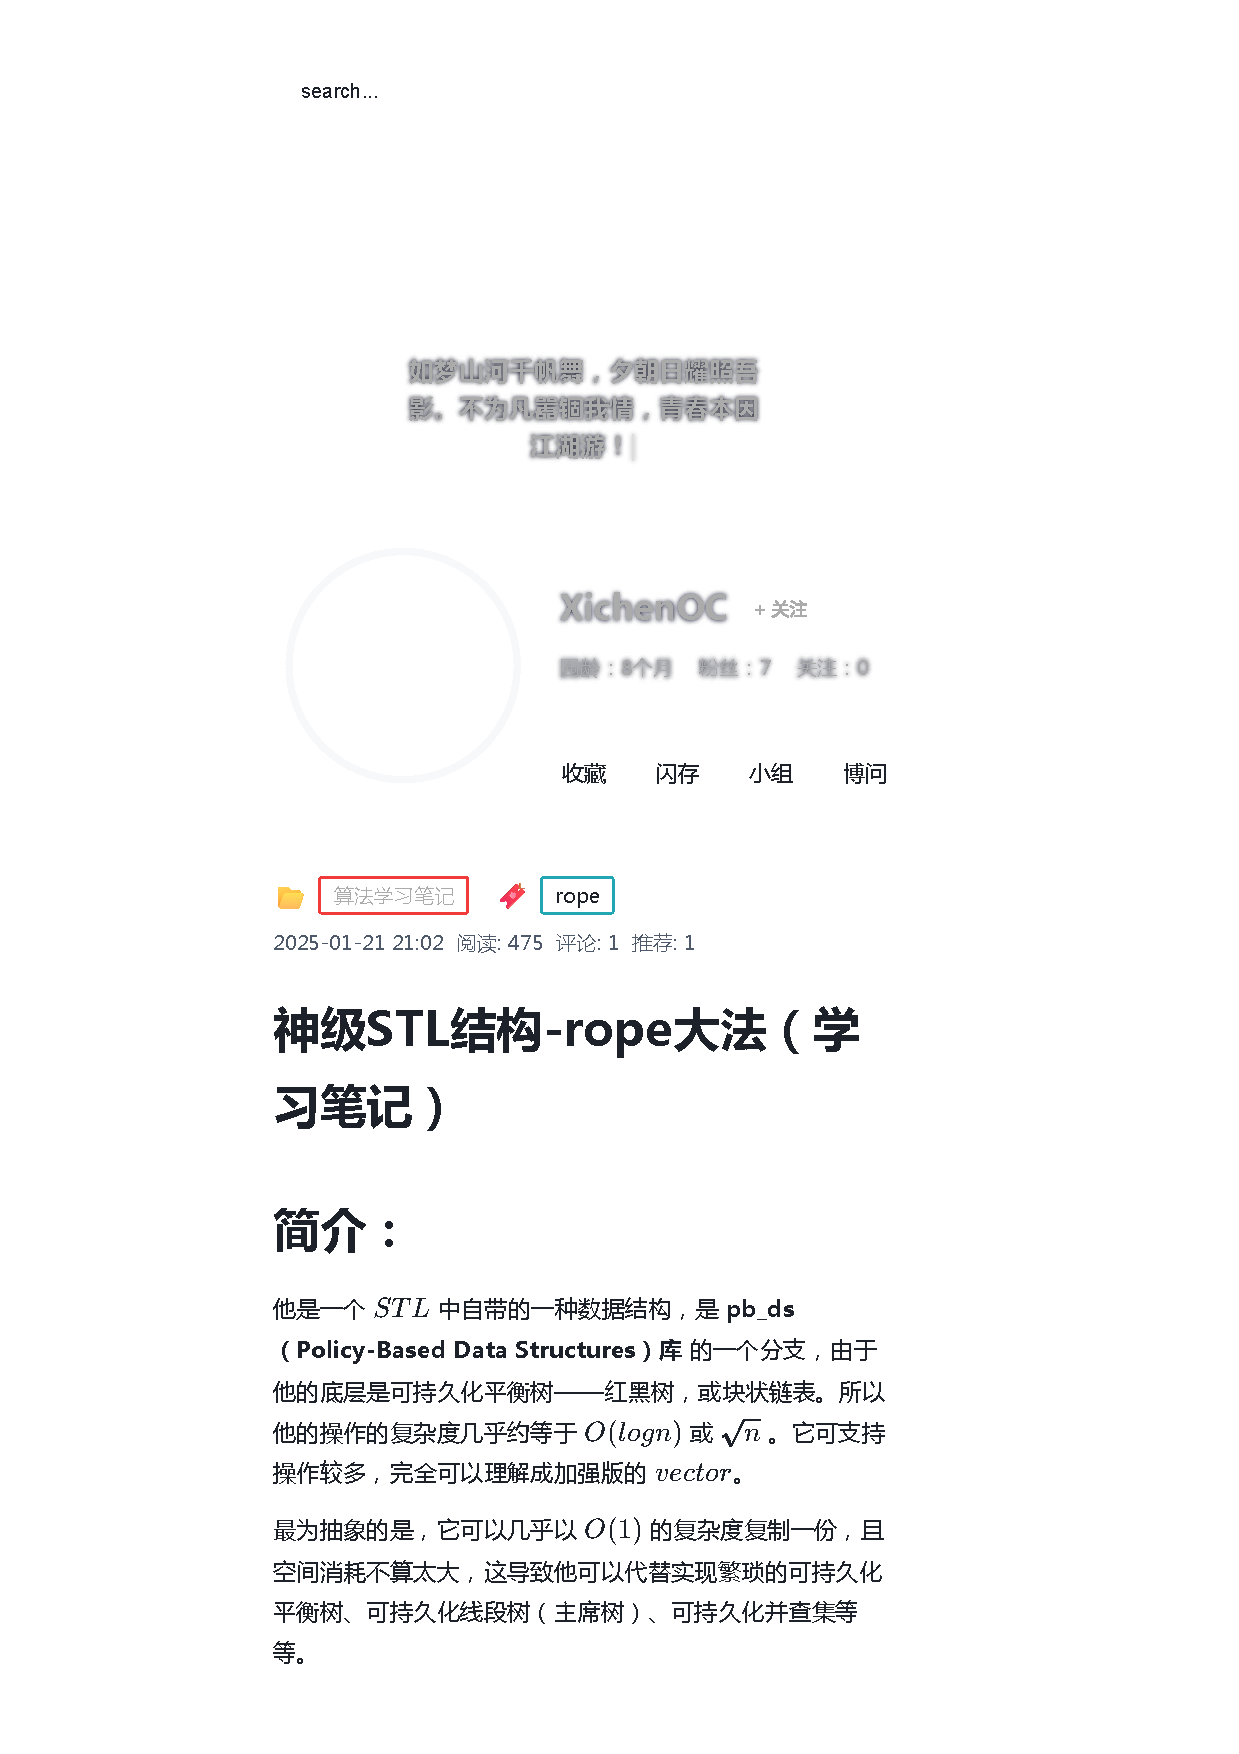
\includegraphics[page=1,width=0.94\linewidth,height=0.90\textheight,keepaspectratio]{assets/pdf/pdf_073.pdf}
\end{center}
\clearpage
\begin{center}
\includegraphics[page=2,width=0.94\linewidth,height=0.90\textheight,keepaspectratio]{assets/pdf/pdf_073.pdf}
\end{center}
\clearpage
\begin{center}
\includegraphics[page=3,width=0.94\linewidth,height=0.90\textheight,keepaspectratio]{assets/pdf/pdf_073.pdf}
\end{center}
\clearpage
\begin{center}
\includegraphics[page=4,width=0.94\linewidth,height=0.90\textheight,keepaspectratio]{assets/pdf/pdf_073.pdf}
\end{center}
\clearpage
\begin{center}
\includegraphics[page=5,width=0.94\linewidth,height=0.90\textheight,keepaspectratio]{assets/pdf/pdf_073.pdf}
\end{center}
\clearpage
\begin{center}
\includegraphics[page=6,width=0.94\linewidth,height=0.90\textheight,keepaspectratio]{assets/pdf/pdf_073.pdf}
\end{center}
\clearpage

\section{数据生成器与对拍}
\entrymeta{—}
\begin{codeline}
const string CHECKER = "checker";
const string TGT = "U224067";

/*
 * 生成闭区间[a,b]内的随机整数
 */
int64 randint(int64 a, int64 b) {
    int64 g = b - a + 1;
    int64 rand64 = 0;
    for(int i = 0; i < 4; i++) {
        rand64 <<= 16;
        rand64 ^= rand();
    }
    return a + rand64 % g;
}

/*
 * 生成T组规模为N的测试数据
 */
string generate_data(int64 T, int64 N) {
    string output;
    int64 n = randint(1, N);
    int64 m = randint(1, N);
    output += to_string(n) + " " + to_string(m) + "\n";

    for(int64 j = 0; j < n; j++) {
        int64 a = randint(1, m);
        int64 b = randint(1, N);
        output += to_string(a) + " " + to_string(b) + "\n";
    }

    return output;
}

/*
 * 比较两个输出文件的内容
 */
bool compare_files(const string& file1, const string& file2) {
    ifstream f1(file1);
    ifstream f2(file2);
    if(!f1.is_open() || !f2.is_open()) {
        cerr << "无法打开输出文件进行比较" << endl;
        return false;
    }
    string line1, line2;
    int64 lineNum = 0;
\end{codeline}
\vspace{-0.9\baselineskip}
\begin{codeline}[firstnumber=47]
    while(getline(f1, line1) && getline(f2, line2)) {
        lineNum++;
        if(line1 != line2) {
            cout << "第 " << lineNum << " 行不一致:" << endl;
            cout << "Ans: " << line1 << endl;
            cout << "Res: " << line2 << endl;
            f1.close();
            f2.close();
            return false;
        }
    }
    if(getline(f1, line1) || getline(f2, line2)) {
        cout << "文件长度不一致" << endl;
        f1.close();
        f2.close();
        return false;
    }
    f1.close();
    f2.close();
    return true;
}

int main() {
    srand(time(0)); // 初始化随机种子

    int64 T = 1;
    int64 N = 2000;

    while(true) {
        string data = generate_data(T, N);
        ofstream f_in("in.in");
        f_in << data;
        f_in.close();

        string cmd1 = CHECKER + " < in.in > outc.out";
        system(cmd1.c_str());

        auto start = chrono::high_resolution_clock::now();
        string cmd2 = TGT + " < in.in > outtgt.out";
        system(cmd2.c_str());
        auto end = chrono::high_resolution_clock::now();
        chrono::duration<double> elapsed = end - start;

        if(compare_files("outc.out", "outtgt.out")) {
            cout << "Accepted! \n运行时间: " << elapsed.count() << " 秒" << endl;
        } else {
\end{codeline}
\vspace{-0.9\baselineskip}
\begin{codeline}[firstnumber=93]
            break;
        }
    }
    return 0;
}
\end{codeline}
\begin{warnbox}
随机种子可复现；每轮对拍前清空输出文件，并检查 \texttt{system()} 返回值。
\end{warnbox}

